\chapter{Resultados e discussões}

Neste capítulo são apresentados os resultados deste trabalho. De modo a manter a coerência dos raciocínios desenvolvidos na defesa desta tese, os resultados não são agrupados de acordo com as técnicas utilizadas, mas sim de acordo com tópicos que representam etapas do trabalho. Os resultados não são apresentados cruamente, sendo acompanhadas de discussões pontuais. Discussões gerais, que são somente possíveis após a exposição do conjunto geral de resultados, são apresentadas na seção \ref{sec:discussao}.

% \ref{sec:expprelim}
% \ref{sec:pre_particao}
% \ref{sec:micros}
% \ref{sec:termodinamica_particao}
% \ref{sec:modelo_cinetico}

Salvo menção contrária, os valores em porcentagem expressos neste capítulo se referem à base de cálculo em massa.

\section{Experimentos preliminares}

\label{sec:expprelim}

Na Figura \ref{fig:thermocalc}a é mostrada a variação das frações molares das fases em equilíbrio calculadas para a liga estudada. O gráfico foi determinado por cálculos termodinâmicos com o software Thermo-Calc\textregistered{} utilizando o banco de dados TCFE. Foram considerados no cálculo apenas os principais elementos presentes na elaboração da liga, Fe, C, Si, Mn e Cu.

Percebe-se que, em consequência do alto teor de carbono da liga, a grafita é presente em toda faixa de temperaturas considerada no cálculo. Por este motivo, durante a austenitização do material, necessariamente a grafita coexistirá em equilíbrio com a austenita. Neste trabalho, a terminologia ``austenitização plena'' é utilizada para descrever a etapa de austenitização neste campo de duas fases, sendo que os cálculos termodinâmicos apontam que essa condição é obtida em temperaturas superiores a \SI{814}{\degreeCelsius}. Entre \SI{814}{\degreeCelsius} e \SI{782}{\degreeCelsius} é prevista a existência de um campo de três fases, denominado ``campo intercrítico'', no qual é estabelecido o equilíbrio termodinâmico entre as fases ferrita (cúbica de corpo centrado), austenita (cúbica de fases centradas) e grafita.

\begin{figure}
  \centering
  \subfloat[]{\includegraphics[width=.48\textwidth]{img/thermo-calc/VPVvsT.pdf}}
  \quad
  \subfloat[]{\includegraphics[width=.48\textwidth]{img/thermo-calc/CvsT.pdf}}
  \caption{Comportamento das frações de fases (a) e teor de carbono dissolvido nas fases em equilíbrio (b) em função da temperatura.}
  \label{fig:thermocalc}
\end{figure}

Na Figura \ref{fig:thermocalc}b é mostrada a variação do teor de carbono dissolvido nas fases em equilíbrio em função da temperatura. Nota-se que temperaturas maiores implicam em uma maior dissolução do carbono na austenita. A \SI{814}{\degreeCelsius}, por exemplo, prevê-se que a austenita possuirá 0,59\%, enquanto que a \SI{900}{\degreeCelsius} a solubilidade do carbono na austenita deverá ser de 0,81\%. Dessa forma, a martensita formada após a têmpera a  partir de temperaturas de austenitização mais elevadas tende a possuir caráter mais frágil devido ao maior teor de carbono, que leva a maior tetragonalidade e maior densidade de discordâncias. Para a faixa de composições de 0,59--0,81\% é esperado que a martensita se apresente predominantemente em morfologia de placas.

De forma a aferir as temperaturas correspondentes aos campos intercrítico e de austenitização plena previstas pelo Thermo-Calc\textregistered{}, realizou-se um experimento de dilatometria para determinar as temperaturas críticas de transformação reais do material.
Na Figura \ref{fig:dil_tempera} é mostrada a curva de dilatação para o ciclo de aquecimento do material. Na curva de dilatação são identificadas quatro distintas regiões (A--D) que apresentam diferentes comportamentos de expansão/contração. Estes diferentes comportamentos são associados à presença de diferentes fases ou ocorrência de transformações de fases.

\begin{figure}
  \subfloat[]{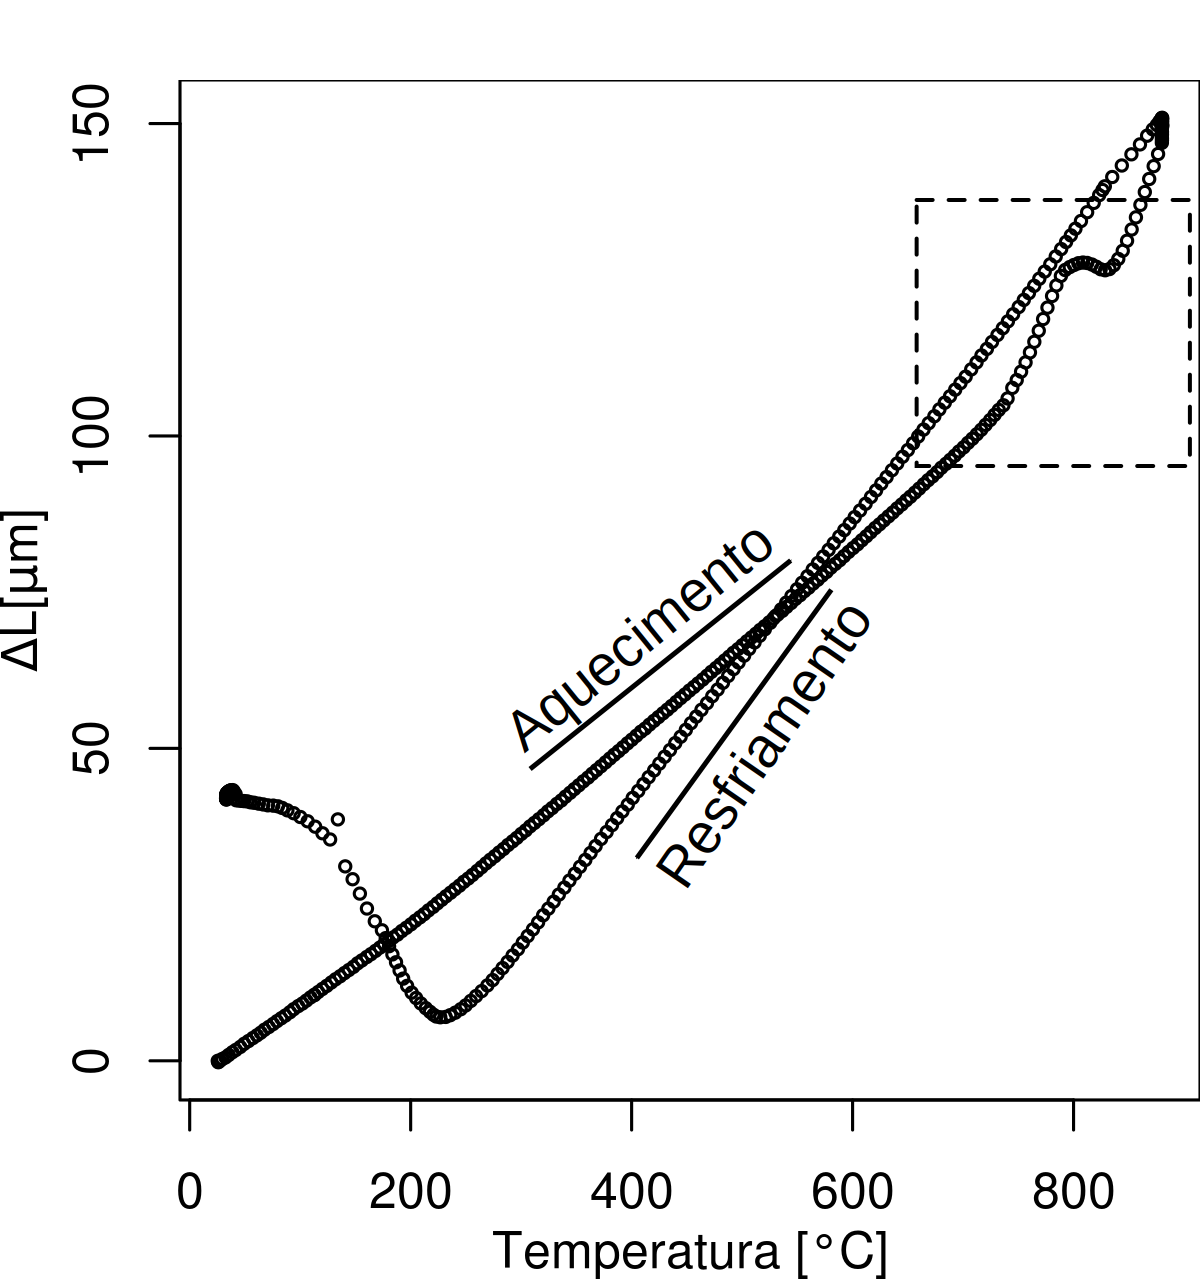
\includegraphics[height=6cm]{img/dilatometria/1_fofoTupy_10oCmin_2.pdf}}
  \quad
  \subfloat[]{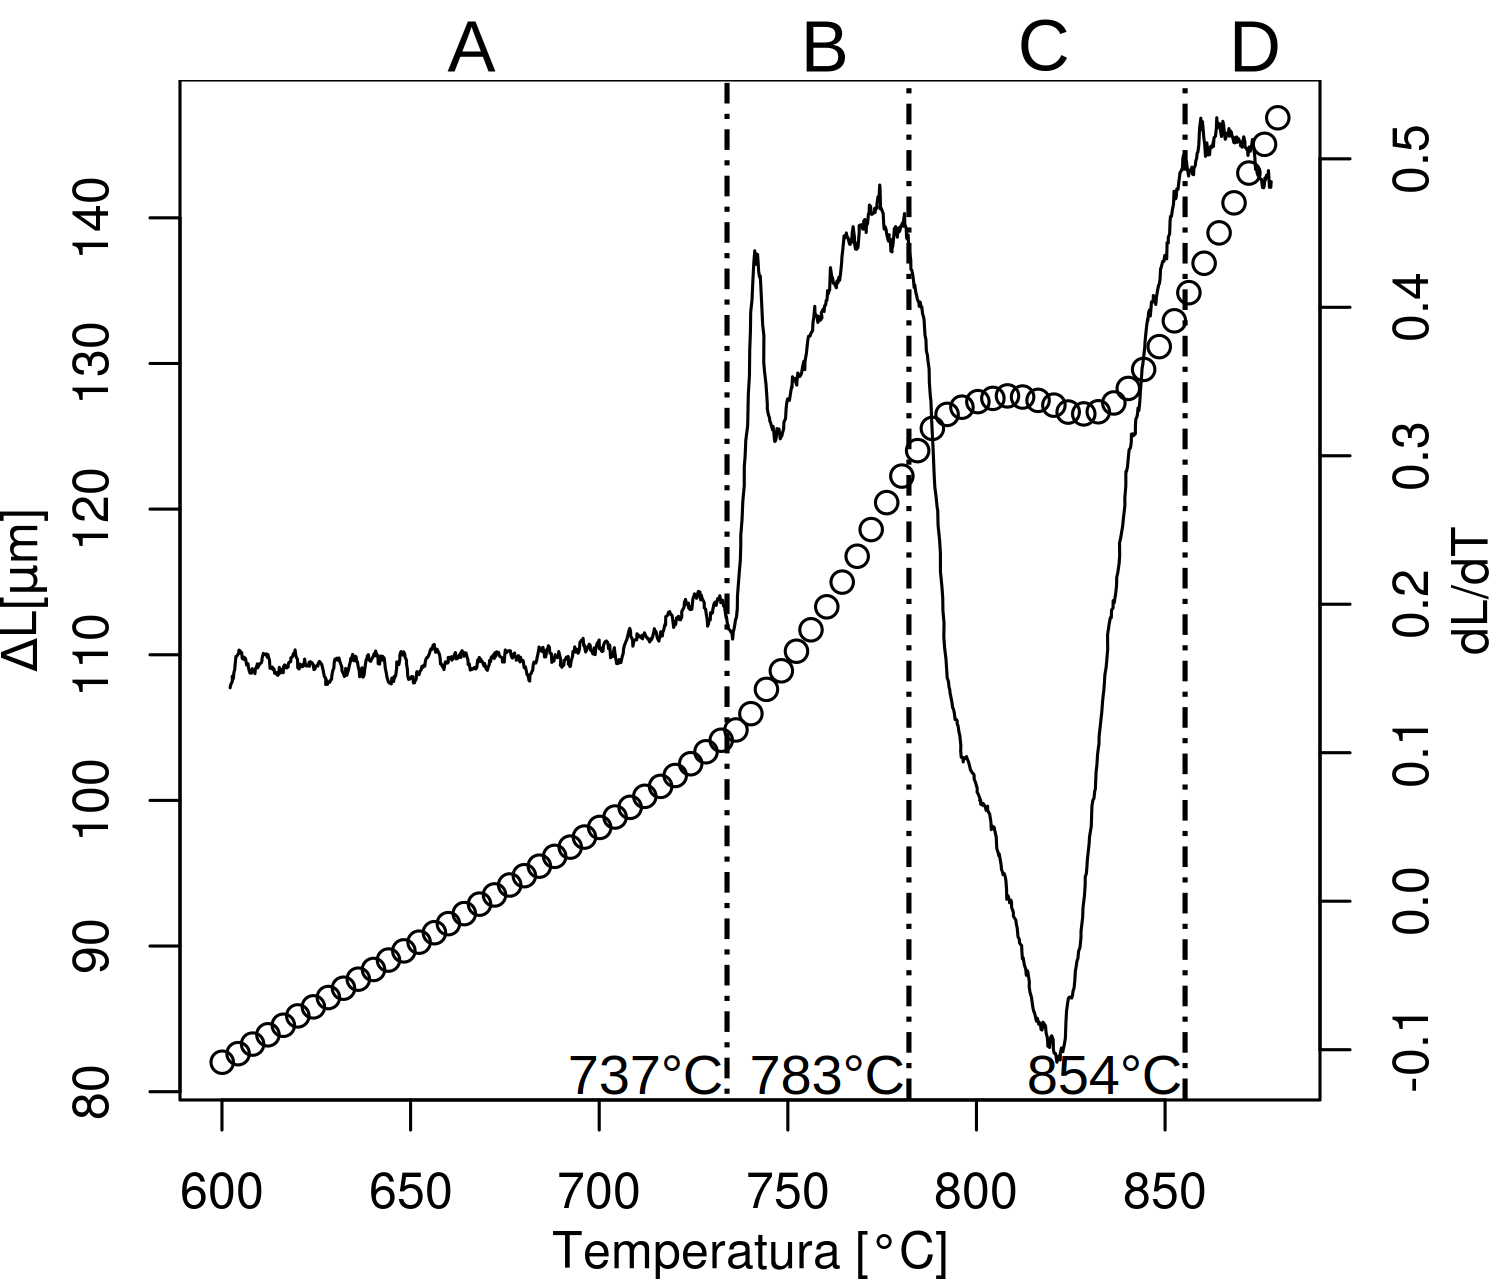
\includegraphics[height=6cm]{img/dilatometria/1_fofoTupy_10oCmin.pdf}}
  \caption{Curva de dilatação em função da temperatura para uma amostra de ferro fundido aquecido a \SI{10}{\degreeCelsius/min} (\SI{0.167}{\degreeCelsius/s}) até a temperatura de \SI{880}{\degreeCelsius}. (a) Curva completa. (b) Detalhe da curva (a) indicado pelo retângulo tracejado. A curva tracejada corresponde à derivada numérica da curva de dilatação em função da temperatura.}
  \label{fig:dil_tempera}
\end{figure}

A microestrutura inicial da amostra ensaiada corresponde à condição como recebida, com dispersão homogênea de nódulos de grafita e matriz ferrítico-perlítica, como mostra a Figura \ref{fig:micro_inicial}. 
Ou seja, o material possui uma combinação de fases metaestáveis (cementita) e estáveis (ferrita e grafita). A interpretação da curva de dilatometria deve levar em conta a condição inicial do material. 
Em temperaturas inferiores a \SI{737}{\degreeCelsius} (região A) o material se dilata de forma aproximadamente linear, condizente com o aumento da agitação térmica. Entre \SI{737}{\degreeCelsius} e \SI{783}{\degreeCelsius} (região B) é observado um aumento da taxa de expansão em relação à etapa anterior. Interpreta-se que esta expansão se origina na dissolução de carbonetos da microestrutura como recebida, levando à formação de grafita. Embora a grafita seja estável para toda a faixa de temperaturas consideradas no ensaio, a baixas temperaturas não há condições cinéticas para dissolução da cementita e formação de grafita.

\begin{figure}
  \subfloat[]{\includegraphics[width=.48\textwidth]{img/micrografias/CR/200x-1_scalebar.pdf}}
  \quad
  \subfloat[]{\includegraphics[width=.48\textwidth]{img/micrografias/CR/500x-2_scalebar.pdf}}
  \caption{Microestrutura do material como recebido apresentando matriz ferrítico-perlítica.}
  \label{fig:micro_inicial}
\end{figure}

Entre \SI{783}{\degreeCelsius} e \SI{854}{\degreeCelsius} (região C) é observada uma contração do material. Esta resposta é associada à formação da fase compacta austenita a partir da ferrita, grafita e cementita não-dissolvida. A partir de \SI{854}{\degreeCelsius} (região D) a dilatação do material volta a ser aproximadamente linear, sinalizando que a formação de austenita tenha cessado.

As temperaturas de transformação determinadas pelo ensaio de dilatometria diferem das temperaturas preditas pela simulação termodinâmica. Essas diferenças podem ser explicadas por alguns fatores, dentre eles:

\begin{itemize}
  \item A microestrutura inicial da amostra de dilatometria não é de equilíbrio. A presença de cementita leva à observação de transformações correspondentes ao eutetóide metaestável.
  \item Embora uma taxa de aquecimento razoavelmente lenta (\SI{10}{\degreeCelsius/min}) tenha sido utilizada, questões cinéticas ainda governam as transformações de fases. A nucleação e crescimento de grãos de austenita a partir da matriz depende da existência de uma força motriz na forma de um sobreaquecimento. Dessa forma, durante o aquecimento contínuo há a tendência de que as temperaturas de transformação sejam mais elevadas do que as temperaturas de equilíbrio. % CITATION NEEDED
  \item A microsegregação interente ao ferro fundido produz regiões com diferentes concentrações de elementos, causando a alteração local das temperaturas de transformação.
\end{itemize}

% Quando comparada com os resultados da simulação termodinâmica, a interpretação da curva de dilatação mostra uma relação coerente entre a temperatura inferior do campo intecrítico (\SI{782}{\degreeCelsius} pelo Thermo-Calc\textregistered{} e \SI{783}{\degreeCelsius} pela dilatometria), mas mostra uma discrepância entre as temperaturas de austenitização plena obtidas pelos dois métodos (\SI{814}{\degreeCelsius} pelo Thermo-Calc\textregistered{} e \SI{854}{\degreeCelsius} pela dilatometria). Essa diferença pode ser justificada pela microsegregação do ferro fundido, que produz regiões com menor concentração de elementos gamagênicos, elevando localmente a temperatura de austenitização plena.
%Outra possibilidade é a própria inabilidade do banco de dados TCFE prever acuradamente o equilíbrio termodinâmico em sistemas complexos, uma vez que o software realiza extrapolações de informações termodinâmicas para prever os potenciais químicos dos elementos.

Dessa forma, é razoável utilizar os resultados de dilatometria para escolha da temperatura de austenitização do material. Por outro lado, os resultados da simulação termodinâmica podem ser utilizados, por exemplo, para determinação da composição média da austenita na temperatura de austenitização.

Uma menor temperatura de austenitização leva a uma austenita com menos carbono, implicando em uma martensita de caráter menos frágil do que a obtida em temperaturas mais elevadas de austenitização, enquanto temperaturas elevadas beneficiam a diminuição da segregação (homogeneização dos elementos químicos) no material. Procurou-se adotar uma temperatura intermediária, que gerasse uma martensita menos frágil, ao mesmo tempo que parte da heterogeneidade decorrente da segregação pudesse ser eliminada. Dado o exposto, foi escolhida a temperatura de austenitização de \SI{880}{\degreeCelsius} para os experimentos subsequentes. Nesta temperatura, a composição química média da austenita prevista por cálculos termodinâmicos é mostrada na Tabela \ref{tab:CQaust}.

\begin{table}
  \caption{Composição química da austenita determinada por cálculo termodinâmico no software Thermo-Calc\textregistered{}.}
  \begin{tabular}{c c c c c}
  \thickhline
  \textbf{Elemento} & C & Si & Mn & Cu\\
  \hline
  \textbf{Composição (\% massa)} & 0,76 & 2.54 & 0,21 & 0,39\\
  \thickhline
  \end{tabular}
  \label{tab:CQaust}
\end{table}

\section{Características microestruturais pré etapa de partição}

\label{sec:pre_particao}

\subsection{Cinética da transformação martensítica}

A Figura \ref{fig:dil_martensita}a mostra a curva de dilatação durante a etapa de têmpera do ensaio de dilatometria utilizado para determinação da temperatura Ms. A expansão observada durante o resfriamento em torno de \SI{230}{\degreeCelsius} corresponde à temperatura de início da transformação martensítica (Ms). 
% Essa conclusão é possível sob o pressuposto de que a taxa de resfriamento de 50~°C/s é suficientemente rápida para garantir que a decomposição difusional da austenita seja evitada. Análise metalográfica posterior (ver seção \ref{sec:micros}) confirma essa observação.
Na mesma figura, a curva tracejada representa a dilatação durante o reaquecimento da mesma amostra após esta ser submetida a imersão em nitrogênio líquido. Este procedimento visa garantir que a transformação martensítica seja completa, de modo que a resposta dilatométrica durante o reaquecimento represente a expansão térmica do material 100\% martensítico.

\begin{figure}
  \subfloat[]{\includegraphics[height=6.5cm]{img/dilatometria/dil_martensita.pdf}}
  \vspace{0pt}
  \subfloat[]{\includegraphics[height=6.5cm]{img/dilatometria/dil_martensita_close.pdf}}
  \caption{Curva de dilatação obtida durante o ciclo de austenitização e têmpera. (a) Curva completa. (b) Detalhe da expansão linear decorrente da transformação martensítica.}
  \label{fig:dil_martensita}
\end{figure}

A Figura \ref{fig:dil_martensita}b mostra em detalhe a dilatação associada à reação martensítica. Em temperaturas superiores à Ms, a matriz do material é completamente austenítica. A dilatação da amostra nesta faixa de temperaturas é aproximadamente linear e é atribuída à agitação térmica. Em temperaturas inferiores à Ms a transformação martensítica é acompanhada de expansão da amostra. A fração transformada de martensita $f^{\alpha'}$ é calculada pela regra das alavancas, expressa pela equação:

\begin{equation}
  f^{\alpha'} = 1 - f^\gamma = \frac{A}{A + B}
  \label{eq:alavanca}
\end{equation}
%
em que $f^\gamma$ é a fração não transformada de austenita. A determinação dos parâmetros ``A'' e ``B'' é feita pela construção mostrada na Figura \ref{fig:dil_martensita}b. $A$ consiste da expansão associada à formação de martensita na temperatura $T_T$ caso o corpo de prova permanecesse 100\% austenítico antes da transformação. Esse comprimento é determinado pela extrapolação do trecho de expansão térmica linear da austenita para a temperatura $T_T$. Por sua vez, $A + B$ é a expansão do corpo de prova caso a amostra se transformasse completamente em martensita na temperatura $T_T$. A determinação de $B$ é feita calculando-se o comprimento extrapolado do material 100\% martensítico (curva tracejada), como mostra a construção na figura.

A fração transformada de martensita em função da temperatura de têmpera é mostrada na Figura \ref{fig:KMFoFo}. Os dados experimentais foram ajustados segundo o modelo proposto por Koistinen e Marburger (equação \ref{eq:KM}) de modo a se ter uma maneira rápida de se avaliar a fração transformada de martensita:

\begin{equation}
  f^{\alpha'} = 1 - f^\gamma = 1 - \exp\left[ -1,217 \times 10^{-2} \left( 216,2 - T_T \right) \right]
\end{equation}

Na equação obtida, os parâmetros de ajuste assumem os valores \linebreak$\beta$ = \SI{1.217e-2}{\degreeCelsius^{-1}} e Ms' = \SI{216.2}{\degreeCelsius}. Nota-se que o parâmetro Ms' assume um valor inferior à temperatura Ms real do material. Essa diferença é reportada na literatura e é decorrente da inércia para desencadeamento dos \enfase{bursts} de martensita na austenita\cite{VanBohemen2008}. Também se percebe que o coeficiente $\beta$ se mostrou bastante próximo ao valor de \SI{1.1e-2}{\degreeCelsius^{-1}} obtido no trabalho original de Koistinen e Marburger\cite{Koistinen1959}.

\begin{figure}
  \includegraphics[width=.7\textwidth]{img/dilatometria/frac_martensita.pdf}
  \caption{Fração não transformada de austenita ($f^\gamma$) em função da temperatura de têmpera determinada pelos dados do experimento de dilatometria.}
  \label{fig:KMFoFo}
\end{figure}

Pela equação obtida, prevê-se que cerca de 10\% (em volume) de austenita é retida quando o material é temperado diretamente à temperatura ambiente (\SI{25}{\degreeCelsius}). A Tabela \ref{tab:austRetida} mostra as quantidades de martensita e austenita esperadas nas temperaturas de têmpera programadas nos experimentos deste trabalho.

\begin{table}
  \caption{Porcentagens (em volume) de martensita e austenita para diferentes temperaturas de têmpera.}
  \begin{tabular}{c c c}
  \thickhline
  Temperatura de têmpera ($T_T$) (\SI{}{\degreeCelsius}) & $f^{\alpha'}$ (\%vol.) & $f^\gamma$ (\%vol.)\\
  \hline
  25 & 90,2 & 9,8\\
  140 & 60,4 & 39,6\\ 
  170 & 43,0 & 57,0\\
  200 & 17,9 & 82,1\\
  \thickhline
  \end{tabular}
  \label{tab:austRetida}
\end{table}

\subsection{Distribuição da martensita formada na etapa de têmpera}

A Figura \ref{fig:tempera}a mostra micrografia de um espécime como temperado, sendo observa uma dispersão homogênea de nódulos de grafita. A fração volumétrica de grafita foi determinada por quantificação estereológico como $10.3 \pm 0.5$~\%vol. Na Figura \ref{fig:tempera}b a microstrutura atacada do material temperado mostra que a matriz apresenta martensita em morfologia de placas, típica de ligas de alto carbono. A distribuição do tamanho das placas é heterogênea, sendo as maiores placas tão grandes quanto \SI{30}{\micro\meter} e menores placas observadas entre as maiores. As maiores placas de martensita foram as primeiras a se formarem quando a temperatura Ms é atingida durante o resfriamento. As placas menores se formaram sob super-resfriamentos maiores preenchendo as regiões de austenita não-transformada entre as placas de martensita pré-existentes.

\begin{figure}
  \centering
  \subfloat[]{\includegraphics[width=.48\textwidth]{img/micrografias/Q/100x-1.pdf}}\quad
  \subfloat[]{\includegraphics[width=.48\textwidth]{img/micrografias/Q/2kx-1_gray.pdf}}
  \caption{Condição como temperada (a) MO, amostra não atacada (b) MEV, amostra atacada com reagente Nital 2\%}
  \label{fig:tempera}
\end{figure}

A microestrutura da amostra temperada a \SI{170}{\degreeCelsius} por 1~min e então resfriada até a temperatura ambiente é mostrada na Figura \ref{fig:temperaInterrompida}a. As placas de martensita com aspecto escurecido devido ao ataque metalográfico revelam a estrutura da martensita antes da etapa de partição. Regiões claras correspondem ao agregado de austenita retida e martensita fresca formada durante o resfriamento final. Este microconstituinte é comumente referido na literatura como MA. A martensita formada durante a primeira etapa de têmpera a a \SI{170}{\degreeCelsius} ($\approx$~43~\%vol.) é ligeiramente revenida durante a etapa isotérmica na etapa de têmpera. Consequentemente esta martensita se comporta diferentemente da martensita presente no microconstituinte MA durante o ataque pelo reagente Nital. Entretanto, como pode ser observado na imagem de MEV desta mesma condição (Figura \ref{fig:temperaInterrompida}b), não há claro indício de precipitação de carbonetos na martensita. É também observado que a distribuição da martensita primária é heterogênea. Regiões próximas a nódulos de grafita apresentam maior fração de martensita revenida, enquanto regiões distantes dos nódulos quase não apresentam martensita. Este comportamento é explicado por mudanças locais na temperatura Ms devido à microssegregação formada durante a solidificação.

\begin{figure}
  \centering
  \subfloat[]{\includegraphics[width=.48\textwidth]{img/micrografias/Q170-1min/500x-1.pdf}}\quad
  \subfloat[]{\includegraphics[width=.48\textwidth]{img/micrografias/Q170-1min/5kx-4_scalebar.pdf}}
  \caption{Microestrutura da amostra temperada a \SI{170}{\degreeCelsius} e mantida por 1~min. (a) MO; (b) MEV. Na imagem de MO, martensita primária ($\alpha'$) é observada como placas escurecidas, enquanto regiões claras correspondem ao microconstituinte MA. Na imagem de MEV, $\alpha'$ aparece em baixo relevo e o MA sob alto relevo.}
  \label{fig:temperaInterrompida}
\end{figure}

A microssegregação foi quantificada por Análise de Microssonda Eletrônica (EPMA) em uma amostra temperada a \SI{170}{\degreeCelsius} e particionada a \SI{375}{\degreeCelsius} por 15~min. Figuras \ref{fig:EPMA}a--c mostram os mapas de composição dos elementos Si, Mn e Cu, respectivamente. Uma vez que a temperatura de partição é relativamente baixa e o tempo de partição curto, a redistribuição dos elementos substitucionais é desprezível nas etapas posteriores à austenitização. Dessa forma, a distribuição de elementos de liga na condição de análise deve ser compatível com a condição temperada e os demais tratamentos T\&P. Tons de cores representam a porcentagem em peso de cada elemento, como indicada pela escala de cor na parte inferior de cada figura. Em todos os mapas os nódulos de grafita se apresentam em tons de azul, uma vez que a grafita possui virtualmente solubilidade zero destes elementos. Regiões próximas aos nódulos de grafita apresentam maiores teores de Si e Cu, enquanto o Mn segrega para regiões de contornos de célula eutética, as últimas regiões a se solidificar. Este comportamento pode ser melhor visualizado no perfil de composições em linha mostrado na Figura \ref{fig:EPMA}d. Considerando apenas a região da matriz do material, a composição de Si varia entre 1.72--2.89~\% e o Mn varia entre 0.19--0.38~\%.

\begin{figure}
  \centering
  \includegraphics[width=.9\textwidth]{img/EPMA/EPMA.pdf}
  \caption{Distribuição das composições dos elementos substitucionais (a) Si, (b) Mn, (c) Cu. (d) Perfis de composição medidos ao longo da linha tracejada desenhada sobre os mapas de composição.}
  \label{fig:EPMA}
\end{figure}

O comportamento da microssegregação destes elementos no ferro fundido é associado às diferentes solubilidades de cada elemento nas fases líquida e sólida (austenita) durante a solidificação. Este comportamento pode ser entendido por meio de simulações Scheil. A Figura \ref{fig:scheil} mostra a evolução da composição da austenita durante a solidificação calculada segundo o método Scheil no software Thermo-Calc\textregistered{}. Percebe-se que para super-resfriamentos crescentes (temperaturas menores) as solubilidades de C e Mn na austenita aumentam, enquanto que as solubilidades de Si e Cu diminuem. Essas diferenças de solubilidade são mais evidentes durante a etapa de solidificação eutética. Dessa forma, os grãos de austenita formados primeiro --- a temperaturas mais altas --- tendem a possuir composição mais próxima à composição média da liga. As últimas regiões a se solidificar, isto é, a temperaturas mais baixas e que vem a se tornar os contornos de célula eutética, formam-se com maiores teores de C e Mn e menores teores de Si e Cu.
 
\begin{figure}
  \centering
  \includegraphics[width=.8\textwidth]{img/thermo-calc/scheil_austenita.pdf}
  \caption{Evolução da composição da fase líquida durante a solidificação da liga calculada pelo método Scheil no software Thermo-Calc\textregistered{}.}
  \label{fig:scheil}
\end{figure}

A distribuição de carbono não foi medida diretamente por EPMA, mas foi determinada utilizando cálculos termodinâmicos e é mostrada no perfil de composição na Figura \ref{fig:EPMA}d. Devido à alta mobilidade do carbono é razoável assumir que após a austenitização a \SI{880}{\degreeCelsius} o potencial químico do carbono (ou atividade do carbono) é homogêneo ao longo da austenita. Sob essa consideração, o potencial químico do carbono $\mu_C$ para a composição média da liga foi determinado utilizando cálculos termodinâmicos. Usando o valor de $\mu_C$ calculado e o conjunto de composições de Si, Mn e Cu determinados por EPMA, cálculos termodinâmicos foram conduzidos de forma a determinar a concentração local de carbono. Como mostrado na Figura \ref{fig:EPMA}d, o carbono apresenta maior concentração próximo aos contornos de célula (0,87~\%) do que nas proximidades dos nódulos de grafita (0,71~\%), assim como ocorre com o Mn.

Tendo a descrição completa das composições de C, Mn, Si e Cu no material após a austenitização, a variação da temperatura Ms de acordo com as variações de composição foram determinadas utilizando a seguinte equação empírica para a temperatura Ms\cite{VanBohemen2012}:

\begin{equation}
  Ms\,(\SI{}{\degreeCelsius}) = 565 - 600 \left[1 - \exp \left( -0.96 \%w_C^\gamma \right)\right] - 31 \%w_{Mn}^\gamma - 13 \%w_{Si}^\gamma
  \label{eq:MsVanBohemen}
\end{equation}
%
em que $\%w_j^\gamma$ é a porcentagem em massa do elemento $j$ dissolvido na austenita. A temperatura Ms calculada para a composição média da austenita é \SI{215}{\degreeCelsius}, abaixo da temperatura Ms experimental determinada por dilatometria, mas de acordo com a temperatura Ms' que aparece na equação de Kostinen-Marburger obtida pelo ajuste dos dados de dilatometria.
Subsequentemente, a temperatura Ms calculada para cada conjunto de composições foi substituída no lugar do parâmetro Ms' na equação \ref{eq:KM}. As equações modificadas foram então utilizada para estimar a fração local de martensita a uma determinada temperatura de têmpera. 

% Figuras xxa--c mostram as distribuições de martensita esperadas após têmpera a 140, 170 e \SI{200}{\degreeCelsius}, respectivamente.
A Figura \ref{fig:EPMA_fmart} mostra a distribuição de martensita $f^{\alpha'}$ calculada para a temperatura de têmpera de \SI{170}{\degreeCelsius}. A fração de martensita em contornos de célula eutética é prevista para ser próxima de zero, de acordo com as observações microestruturais mostradas na Figura \ref{fig:temperaInterrompida}a. Histogramas mostrados na Figura \ref{fig:EPMA_fmart}b descrevem as distribuições estatísticas de martensita na matriz do ferro fundido temperado a 25, 140, 170 e \SI{200}{\degreeCelsius}. A fração média de martensita --- representada pelas linhas tracejadas verticais --- estão de acordo com os valores previstos pela aplicação da equação de Kostinen-Marburger (eq. \ref{eq:KM}). Percebe-se que as distribuições são mais largas quanto maior a temperatura de têmpera. Isto significa que temperaturas mais baixas de têmpera levam a uma distribuição mais homogênea de martensita na matriz do material, parcialmente diminuindo os efeitos da microssegregação de elementos.

\begin{figure}
  \centering
  \includegraphics[width=.9\textwidth]{img/EPMA/EPMA_fmart.pdf}
  \caption{(a) Fração local de martensita $f^{\alpha'}$ prevista após têmpera a \SI{170}{\degreeCelsius}. (b) Histogramas da distribuição de $f^{\alpha'}$ após têmpera a 25, 140, 170 e \SI{200}{\degreeCelsius}. Linhas tracejadas indicam o valor médio de $f^{\alpha'}$. Valores entre parênteses correspondem ao desvio padrão da distribuição.}
  \label{fig:EPMA_fmart}
\end{figure}

%%%%%%%%%%%%%%%%%%%%%%

\section{Características microestruturais das amostras temperadas e particionadas}

\label{sec:micros}

% A evolução microestrutural do material temperado e particionada é avaliada nesta seção de acordo com três variáveis de tratamento térmico. Na seção \ref{sec:micros_tempo} é apresentado o efeito de tempos crescentes de partição na microestrutura do material temperado a \SI{170}{\degreeCelsius} e particionado a \SI{375}{\degreeCelsius}. Na seção \ref{sec:micros_TP} é feita uma avaliação sobre as mudanças microestruturais observadas para diferentes temperaturas de partição. Por fim, na seção \ref{sec:micros_TT} 

% \subsection{Efeito do tempo de partição na microestrutura final}

% \label{sec:micros_tempo}

\subsection{Efeito da temperatura de partição na microestrutura final}

\label{sec:micros_TP}

Nas figuras \ref{fig:TP375MO}a--d são mostradas imagens de microscopia óptica das amostras temperadas a \SI{170}{\degreeCelsius} e particionadas a \SI{375}{\degreeCelsius} por 0, 30~s e, 5~min e 15~min. 
Sob baixa magnificação ($200\times$) podem ser distinguidas regiões escuras, atacadas pelo reagente Nital, e regiões claras, não-atacadas. As regiões não-atacadas correspondem a regiões de MA, isto é, o agregado de austenita retida e martensita formada durante o resfriamento final (martensita fresca, $\alpha'_{fr}$). Antes do resfriamento final as regiões de MA correspondiam a áreas em que a austenita não sofreu transformação durante as etapas do processo T\&P.

\begin{figure}
  \centering
  \subfloat[]{\includegraphics[width=.48\textwidth]{img/micrografias/170-375/MO/QP0_scalebar.pdf}}
  \quad
  \subfloat[]{\includegraphics[width=.48\textwidth]{img/micrografias/170-375/MO/QP30s_scalebar.pdf}}
  \vspace{0pt}
  \subfloat[]{\includegraphics[width=.48\textwidth]{img/micrografias/170-375/MO/QP5min_scalebar.pdf}}
  \quad
  \subfloat[]{\includegraphics[width=.48\textwidth]{img/micrografias/170-375/MO/QP15min_scalebar.pdf}}
  \caption{Imagens de MO das amostras temperadas por \SI{170}{\degreeCelsius} e particionadas a \SI{375}{\degreeCelsius} por (a) 0~s, (b) 30~s, (c) 5~min, (d) 15~min.}
  \label{fig:TP375MO}
\end{figure}

Fica claro que as regiões de MA se encontram preferencialmente nas regiões de contorno de célula. Este comportamento é explicado pelo efeito da microsegregação de elementos de liga na temperatura Ms local, como discutido anteriormente.
Regiões de contornos de célula contendo MA, correspondentes às condições de partição por 0 e 30~s, são mostradas em detalhe na Figura \ref{fig:TP375MO_1000x}. Nota-se a presença de pequenos produtos aciculares nestas regiões principalmente a 30~s, indicando as etapas iniciais de uma reação competitiva de decomposição da austenita. Com o aumento do tempo de partição, as regiões de contorno de célula, antes ricas em MA, passam a apresentar o padrão de ataque observado no restante da amostra, denotando a decomposição isotérmica da austenita durante a etapa de partição. 
A identificação microestrutural individual das fases é dificilmente realizada por MO. Dessa forma, observações por microscopia eletrônica de varredura foram realizadas para esta finalidade.

\begin{figure}
  \centering
  \subfloat[]{\includegraphics[width=.48\textwidth]{img/micrografias/170-375/MO/QP0_1000x_scalebar.pdf}}
  \quad
  \subfloat[]{\includegraphics[width=.48\textwidth]{img/micrografias/170-375/MO/QP30s_1000x_scalebar.pdf}}
  \caption{Imagens de MO em alta magnificação ($1000 \times$) das amostras temperadas por \SI{170}{\degreeCelsius} e particionadas por \SI{375}{\degreeCelsius} por (a) 0~s e (b) 30~s.}
  \label{fig:TP375MO_1000x}
\end{figure}

% temperadas a \SI{170}{\degreeCelsius} e particionadas a \SI{375}{\degreeCelsius} por 0, 30~s e, 5~min e 15~min.
As figuras \ref{fig:TP375-0_MEV}--\ref{fig:TP375-15min_MEV} mostram imagens de MEV das mesmas amostras observadas por MO.
Sob o MEV, os aspectos microestruturais identificados incluem placas de martensita ($\alpha'$) atacadas, aquelas formadas durante a etapa de têmpera, com clara presença de carbonetos precipitados internamente. Neste texto, os carbonetos de revenimento são denotados pelo símbolo $\theta$. Percebe-que mesmo para o tempo mais curto de partição (0~s, ou seja, temperado imediatamente após a temperatura de partição ser atingida, Figura \ref{fig:TP375-0_MEV}) é observado um aspecto superficial na martensita significantemente diferente daquele observado na amostra temperada a \SI{170}{\degreeCelsius}, mas não particionada (Figura \ref{fig:temperaInterrompida}). Isto fica mais claro sob maior magnificação (Figura \ref{fig:TP375-0_MEV}b). Na espinha central da placa (\enfase{midrib}) podem ser observadas linhas paralelas perpendiculares à espinha, associadas às maclas de deformação formadas para acomodar a transformação. Não fica claro pelas imagens de MEV se há carbonetos precipitados na \enfase{midrib}. Por outro lado, no restante da placa, que possui menor densidade de maclas, é possível observar um padrão de ataque distintivo de carbonetos orientados em diferentes direções. Ao aumentar o tempo de partição para 5 e 15~min (figuras \ref{fig:TP375-5min_MEV}a--b e \ref{fig:TP375-15min_MEV}a--b) não é aparente qualquer variação na fração de fases de carbonetos dentro da martensita.

Para tempos superiores a 30~s (figuras \ref{fig:TP375-30s_MEV}a--b) é possível observar um produto acicular mais fino do que a martensita. Este microconstituinte é associado ao produto observado por MO nos contornos de célula (ver novamente Figura \ref{fig:TP375MO_1000x}b). A fração deste produto aumenta com o tempo de partição. Pela morfologia, é possível identificar com segurança que este microconstituinte consiste de bainita. Para curtos tempos (30~s e 5~min) não há evidência de precipitação de carbonetos dentro da bainita, de modo que é também possível inferir que para curtos tempos o produto bainítico consiste apenas de ferrita bainítica ($\alpha_b$), derivada da decomposição incompleta da austenita. Devido ao alto teor de silício e temperatura de transformação, é de fato esperado que um produto bainítico isento de carbonetos seja formado nesta temperatura. Ao passo que a fração de $\alpha_b$ aumenta, é visível que uma pequena fração de carbonetos é formada dentro da bainita, mostrando que o segundo estágio da reação bainítica começara.

\begin{figure}
  \centering
  $T_T = \SI{170}{\degreeCelsius}$; $T_P = \SI{375}{\degreeCelsius}$ / \SI{0}{s}\\
  \subfloat[]{\includegraphics[width=.48\textwidth]{img/micrografias/170-375/MEV/0/5kx-3.pdf}}
  \quad
  \subfloat[]{\includegraphics[width=.48\textwidth]{img/micrografias/170-375/MEV/0/20kx-1.pdf}}
  \caption{Imagens de MEV da amostra temperada a \SI{170}{\degreeCelsius} e particionada a \SI{375}{\degreeCelsius} por 0~s.}
  \label{fig:TP375-0_MEV}
\end{figure}

\begin{figure}
  \centering
  $T_T = \SI{170}{\degreeCelsius}$; $T_P = \SI{375}{\degreeCelsius}$ / \SI{30}{s}\\
  \subfloat[]{\includegraphics[width=.48\textwidth]{img/micrografias/170-375/MEV/30s/5a.pdf}}
  \quad
  \subfloat[]{\includegraphics[width=.48\textwidth]{img/micrografias/170-375/MEV/30s/5b.pdf}}
  \vspace{0pt}
  \subfloat[]{\includegraphics[width=.48\textwidth]{img/micrografias/170-375/MEV/30s/5d.pdf}}
  \quad
  \subfloat[]{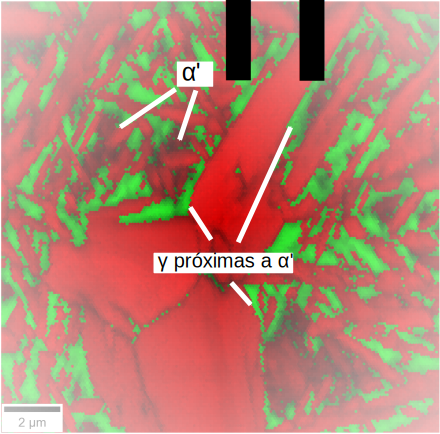
\includegraphics[width=.48\textwidth]{img/micrografias/170-375/MEV/30s/5e.pdf}}
  \caption{Imagens de MEV e mapas de fase obtidos por EBSD da amostra temperada a \SI{170}{\degreeCelsius} e particionada a \SI{375}{\degreeCelsius} por 30~s. Os pares de imagens (a)--(c) e (b)--(d) correspondem às mesmas regiões.}
  \label{fig:TP375-30s_MEV}
\end{figure}

\begin{figure}
  \centering
  $T_T = \SI{170}{\degreeCelsius}$; $T_P = \SI{375}{\degreeCelsius}$ / \SI{5}{min}\\
  \subfloat[]{\includegraphics[width=.48\textwidth]{img/micrografias/170-375/MEV/5min/5kx-6.pdf}}
  \quad
  \subfloat[]{\includegraphics[width=.48\textwidth]{img/micrografias/170-375/MEV/5min/10kx-4.pdf}}
  \caption{Imagens de MEV da amostra temperada a \SI{170}{\degreeCelsius} e particionada a \SI{375}{\degreeCelsius} por 5~min.}
  \label{fig:TP375-5min_MEV}
\end{figure}

\begin{figure}
  \centering
  $T_T = \SI{170}{\degreeCelsius}$; $T_P = \SI{375}{\degreeCelsius}$ / \SI{15}{min}\\
  \subfloat[]{\includegraphics[width=.48\textwidth]{img/micrografias/170-375/MEV/15min/1300x.pdf}}
  \quad
  \subfloat[]{\includegraphics[width=.48\textwidth]{img/micrografias/170-375/MEV/15min/5kx-8.pdf}}
  \vspace{0pt}
  \subfloat[]{\includegraphics[width=.48\textwidth]{img/micrografias/170-375/MEV/15min/QP170-375-15_phase.pdf}}
  \quad
  \subfloat[]{\includegraphics[width=.48\textwidth]{img/micrografias/170-375/MEV/15min/5f.pdf}}
  \caption{Imagens de MEV e mapas de fase obtidos por EBSD da amostra temperada a \SI{170}{\degreeCelsius} e particionada a \SI{375}{\degreeCelsius} por 15~min. Os pares de imagens (a)--(c) e (b)--(d) correspondem às mesmas regiões.}
  \label{fig:TP375-15min_MEV}
\end{figure}

O microconstituinte MA é observado na imagens de MEV na forma das regiões não atacadas em alto relevo.
Para 30~s um grande bloco de MA é observado em uma região de contorno de célula, com menor fração de martensita primária. Isto reflete a distribuição heterogênea de martensita devido à segregação, como discutido anteriormente. Em regiões com maior fração de $\alpha'$, regiões menores de MA são observados entremeados entre as placas de $\alpha'$ e $\alpha_b$. Como resultado do aumento da fração de $\alpha_b$, a fração e o tamanho dos blocos de MA diminuem, tornando-se mais homogeneamente dispersos na matriz, mesmo nas regiões com menor fração de martensita.
Regiões de MA são observadas para todos os tempos, mesmo para os tempos mais longos, o que não havia sido observado por MO. É importante salientar que o microconstituinte MA pode ser constituído completamente de austenita retida, de martensita fresca, ou de uma mistura dos dois. No entanto, apenas pela análise de MEV, é impossível determinar com certeza qual é o caso.
% A presença de ferrita bainítica é claramente um elemento importante na microstrutura do ferro fundido T\&P. A fim de comparação, a Figura xx mostra uma imagem de MEV de uma amostra austemperada a \SI{375}{\degreeCelsius} por 15~min, apresentado uma microestrutura de austenita e ferrita bainítica (ou seja, sem martensita primária). É evidente que a estrutura ba

As imagens das condições 30~s e 15~min são acompanhadas dos respectivos mapas de fase obtidos por EBSD (figuras \ref{fig:TP375-30s_MEV}c--d e \ref{fig:TP375-15min_MEV}c--d). Nos mapas de EBSD, as regiões coloridas em verde representam as fases indexadas com estrutura cúbica de faces centradas (austenita), enquanto as regiões vermelhas correspondem a regiões indexadas como fases cúbicas de corpo centrado (ferrita e martensita). A informação de distribuição de fases é também superposta com a informação de índice de qualidade (IQ) da varredura de EBSD, representada na forma de camada em escala de cinza. Devido às diferenças na concentração de carbono e densidade de discordâncias, os valores de IQ das regiões de $\alpha'_{fr}$ são menores do que nas placas de $\alpha'$, resultando em $\alpha'_{fr}$ aparecendo de forma mais escura do que $\alpha'$. A proporção de $\alpha'_{fr}/\gamma$ nas regiões de MA pode ser observada pela comparação direta dos mapas de fase de EBSD com as imagens de MEV das mesmas regiões. Para 30~s, o grande bloco de MA observado na imagem de MEV é constituído predominantemente de $\alpha'_{fr}$. Por outro lado, os menores blocos de MA constituem-se essencialmente de $\gamma$ retida. É também observado que a maioria da austenita encontrada dentro de blocos de MA está localizada próxima à martensita primária e as placas de ferrita bainítica. Para tempos crescentes a fração de $\alpha'_{fr}$ diminui e a dispersão de $\gamma$ se torna mais homogênea no material.

A estabilização da austenita pelo enriquecimento em carbono é possível por tanto a partição de carbono proveniente da martensita como pela rejeição de carbono durante o crescimento de ferrita bainítica. Em ambos os casos o carbono se acumula na austenita à frente das interfaces e um perfil de carbono transiente é formado. Como consequência, mesmo para curtos tempos de partição a austenita de alto carbono próxima às interfaces é estabilizada durante o resfriamento final.
Revertendo o raciocínio, a presença de austenita retida próxima às placas de martensita, tal qual observado na Figura \ref{fig:TP375-30s_MEV}d, é forte evidência de que a partição de carbono entre martensite e austenita ocorre, mesmo quando carbonetos estão precipitados na martensita.

Imagens de MEV e mapas de fases de EBSD das amostras T\&P particionadas a \SI{300}{\degreeCelsius} por 15~min, \SI{450}{\degreeCelsius} por 30~s e \SI{450}{\degreeCelsius} por 15~min são mostradas nas figuras \ref{fig:TP300-15min_MEV}, \ref{fig:TP450-30s_MEV} e \ref{fig:TP450-15min_MEV}, respectivamente. Com exceção da amostra particionada a \SI{450}{\degreeCelsius} por 15~min, as microestruturas apresentam detalhes similares àqueles das amostras particionadas a \SI{375}{\degreeCelsius}, sendo compostas primariamente de $\alpha'$, $\alpha_b$ e blocos de MA. A comparação das microestruturas produzidas nas três diferentes temperaturas de partição revela que tanto as estruturas de ferrita bainítica, quanto as dimensões dos carbonetos precipitados na martensita são mais refinados quanto menor a temperatura de partição. 

\begin{figure}
  \centering
  $T_T = \SI{170}{\degreeCelsius}$; $T_P = \SI{300}{\degreeCelsius}$ / \SI{15}{min}\\
  % \subfloat[]{\includegraphics[width=.48\textwidth]{img/micrografias/170-outros/6a.pdf}}
  \subfloat[]{\includegraphics[width=.48\textwidth]{img/micrografias/170-outros/300C_5kx-3.pdf}}
  \quad
  \subfloat[]{\includegraphics[width=.48\textwidth]{img/micrografias/170-outros/300C_10kx-1.pdf}}
  \quad
  \caption{Imagens de MEV da amostra temperada a \SI{170}{\degreeCelsius} e particionada a \SI{300}{\degreeCelsius} por 15~min.}
  \label{fig:TP300-15min_MEV}
\end{figure}

\begin{figure}
  \centering
  $T_T = \SI{170}{\degreeCelsius}$; $T_P = \SI{450}{\degreeCelsius}$ / \SI{30}{s}\\
  \subfloat[]{\includegraphics[width=.48\textwidth]{img/micrografias/170-outros/6b.pdf}}
  \quad
  \subfloat[]{\includegraphics[width=.48\textwidth]{img/micrografias/170-outros/6c.pdf}}
  \vspace{0pt}
  \subfloat[]{\includegraphics[width=.48\textwidth]{img/micrografias/170-outros/6d.pdf}}
  \quad
  \caption{Imagens de MEV e mapas de fase obtidos por EBSD da amostra temperada a \SI{170}{\degreeCelsius} e particionada a \SI{450}{\degreeCelsius} por 30~s. As imagens (a) e (b) correspondem às mesmas regiões. A imagem detalhada em (c) evidencia a nucleação de ferrita bainítica em uma interface martensita / austenita}
  \label{fig:TP450-30s_MEV}
\end{figure}

\begin{figure}
  \centering
  $T_T = \SI{170}{\degreeCelsius}$; $T_P = \SI{450}{\degreeCelsius}$ / \SI{15}{min}\\
  \subfloat[]{\includegraphics[width=.48\textwidth]{img/micrografias/170-outros/6e.pdf}}
  \quad
  \subfloat[]{\includegraphics[width=.48\textwidth]{img/micrografias/170-outros/6f.pdf}}
  \quad
  \caption{Imagens de MEV e mapas de fase obtidos por EBSD da amostra temperada a \SI{170}{\degreeCelsius} e particionada a \SI{450}{\degreeCelsius} por 15~min. O mapa de fases em (b) mostra pequena quantidade de austenita retida, quando comparada às demais condições de tratamento de T\&P.}
  \label{fig:TP450-15min_MEV}
\end{figure}

Notavelmente, para a condição de partição a \SI{450}{\degreeCelsius} por 30~s (Figura \ref{fig:TP450-30s_MEV}) é possível observar placas de bainita sendo nucleadas nas interfaces martensita/austenita, sugerindo que a martensita primária desempenha um papel importante assistindo a nucleação de bainita. Este fenômeno será discutido em mais detalhes nas próximas seções. Para a condição $T_P = \SI{450}{\degreeCelsius}$ por 15~min, o mapa de fases de EBSD não revela uma fração apreciável de austenita. Imagens de MEV mostram intensa precipitação de carbonetos em ambas martensita e bainita, indicando que para esta condição a reação bainítica é completa, tendo consumido toda a austenita.

\subsection{Efeito da temperatura de têmpera na microestrutura final}

\label{sec:micros_TT}

As Figuras \ref{fig:TP300MEV} mostram micrografias obtidas por MEV das microestruturas das amostras temperadas a 140, 170 e \SI{200}{\degreeCelsius} e em seguida particionadas a \SI{300}{\degreeCelsius} por 15 minutos. Na análise dos resultados apresentados adiante, a temperatura de partição foi mantida fixa para que a morfologia do produto isotérmico formado durante a partição fosse a mesma para as amostras avaliadas, de modo a levar em conta apenas a influência da temperatura de têmpera. O principal efeito da temperatura de têmpera na evolução microestrutural é o controle da quantidade inicial de martensita e, consequentemente, a quantidade inicial de austenita não-transformada.

Embora os resultados de dilatometria apontem a existência de maiores quantidades de placas de martensita na amostra temperada a \SI{140}{\degreeCelsius} (Figura \ref{fig:TP300MEV}a), essa diferença é pouco perceptível na análise microestrutural. Por outro lado, nota-se uma nítida diferença na dimensão longitudinal dos feixes do produto bainítico. A ferrita bainítica formada após têmpera a \SI{200}{\degreeCelsius} é consideravelmente mais alongada do que aquela formada após têmpera a \SI{170}{\degreeCelsius}, que por sua vez é mais alongada do que a formada após a têmpera a \SI{140}{\degreeCelsius}. Isto é, quanto menor a temperatura de têmpera --- ou seja, quanto maior a quantidade inicial de martensita formada durante a têmpera --- mais refinado é o produto bainítico.

\begin{figure}
  \centering
  \subfloat[$T_T=\SI{140}{\degreeCelsius}$]{\includegraphics[width=.48\textwidth]{img/micrografias/efeito_tempera/140-300-2h.pdf}}
  \quad
  \subfloat[$T_T=\SI{170}{\degreeCelsius}$]{\includegraphics[width=.48\textwidth]{img/micrografias/efeito_tempera/170-300-2h.pdf}}
  \vspace{0pt}
  \subfloat[$T_T=\SI{200}{\degreeCelsius}$]{\includegraphics[width=.48\textwidth]{img/micrografias/efeito_tempera/200-300-2h.pdf}}
  \caption{Imagens de MEV das amostras temperadas a (a) 140, (b) 170 e (c) $T_T$ = \SI{200}{\degreeCelsius} e particionadas \SI{300}{\degreeCelsius} por 2~h. Setas azuis indicam placas de martensita e setas vermelhas indicam a ferrita bainítica ocupando as regiões entre placas de martensita.}
  \label{fig:TP300MEV}
\end{figure}

Este resultado pode ser explicado pela repartição dos grãos originais de austenita pela martensita. Quanto maior a quantidade inicial de martensita (temperaturas de têmpera mais baixas), menor o tamanho de grão da austenita não transformada. Logo, uma vez que o crescimento dos feixes de bainita é limitado pelos contorno de grão --- sejam entre dois grãos de austenita, seja entre uma placa de martensita [ou outro feixe de bainita] e a austenita --- menor a dimensão do produto bainítico formado.

Isso fica ainda mais claro quando as microestruturas das amostras T\&P é comparada com a microestrutura do material submetido ao tratamento de austêmpera (ADI), mostrada na Figura \ref{fig:ADI300MEV}. Note-se que, enquanto os feixes de ferrita bainítica na amostra temperada a \SI{140}{\degreeCelsius} e particionada a \SI{300}{\degreeCelsius} possuem cerca de \SI{5}{\mu m} de comprimento, o feixe de bainita no ADI produzido após austêmpera a \SI{300}{\degreeCelsius} por 15 minutos (Figura \ref{fig:ADI300MEV}) possui aproximadamente \SI{20}{\mu m} de comprimento.

\begin{figure}
  \centering
  \subfloat[]{\includegraphics[width=.48\textwidth]{img/micrografias/ADI/300-15min/2500x-1.pdf}}
  \quad
  \subfloat[]{\includegraphics[width=.48\textwidth]{img/micrografias/ADI/300-15min/10kx-1.pdf}}
  \caption{Imagens de MEV da amostra austemperada a \SI{300}{\degreeCelsius} por 15~min. Nota-se que as dimensões dos feixes de bainita são maiores do que nas T\&P.}
  \label{fig:ADI300MEV}
\end{figure}

% \begin{figure}
%   \centering
%   \subfloat[]{\includegraphics[width=.48\textwidth]{img/micrografias/ADI/375-15min/2kx-1.pdf}}
%   \quad
%   \subfloat[]{\includegraphics[width=.48\textwidth]{img/micrografias/ADI/375-15min/5kx-2.pdf}}
%   \vspace{0pt}
%   \subfloat[]{\includegraphics[width=.48\textwidth]{img/micrografias/ADI/375-15min/ADI375-15_phase.pdf}}
%   \caption{Amostra austemperada a \SI{300}{\degreeCelsius} / 15 minutos. (a) MEV, 2500x. (b) MEV, 10kx. Nota-se que a bainita é ainda mais alongada do que nas amostras T\&P. É possível também ver detalhes da subestrutura dos feixes de bainita, como subunidades e filmes de austenita entre ripas.}
%   \label{fig:ADI375MEV}
% \end{figure}

%%%%%%%%%%%%%%%%%%%%%%

\subsection{Caracterização dos carbonetos precipitados durante T\&P}

A caracterização microestrutural das amostras temperadas e particionadas mostra a presença de carbonetos de revenimento na martensita, mesmo para os tempos mais curtos de partição, indicando que a precipitação de carbonetos ocorre rapidamente durante a etapa de aquecimento da temperatura de têmpera $T_T$ até a temperatura de partição $T_P$. No entanto, a natureza dos carbonetos precipitados, embora possível de ser inferida pelas temperaturas de tratamento, carece de evidência experimental. Nesta seção, os carbonetos precipitados durante o processo T\&P são caracterizados por técnicas de difração.

Experimentos de difração de raios X \enfase{ex situ} utilizando fonte síncrotron foram conduzidos nas seguintes condições:

\begin{itemize}
  \item Amostra temperada à temperatura ambiente
  \item Têmpera a \SI{170}{\degreeCelsius} e partição a \SI{300}{\degreeCelsius} por 2~h
  \item Têmpera a \SI{170}{\degreeCelsius} e partição a \SI{375}{\degreeCelsius} por 2~h
  \item Têmpera a \SI{170}{\degreeCelsius} e partição a \SI{450}{\degreeCelsius} por 2~h
  \item Amostra temperada à temperatura ambiente e revenida por aquecimento contínuo até \SI{700}{\degreeCelsius}
\end{itemize}

Estas aquisições de DRX em particular foram realizadas utilizando o detector 2D Rayonix SX165, em oposição às aquisições \enfase{in situ} feitas utilizando o detector Mythen 1K, cujos resultados são mostrados adiante na seção \ref{sec:DRXInSitu}.

Na Figura \ref{fig:Rayonix_completo} é mostrada a superposição dos difratogramas obtidos para as condições mencionadas acima. Para identificação das fases, também são mostrados as posições esperadas dos picos de difração da ferrita e da austenita. Como a ferrita e a martensita são, do ponto de vista cristalográfico, muito semelhantes, seus respectivos padrões de difração se superpõem. Embora a martensita seja uma fase tetragonal de corpo centrado, a razão de c/a entre seus parâmetros de rede é muito próxima de 1.

\begin{figure}
  \centering
  \includegraphics[width=\textwidth]{img/XTMS/selected_diffractograms.pdf}
  \caption{Difratogramas obtidos por DRX utilizando feixe de luz síncrotron monocromático com comprimento de onda $\lambda = \SI{1.0332}{\text{\AA}}$. As intensidades foram normalizadas pela área integrada do sinal de fundo (proporcional à contagem total de fótons no experimento). As linhas verticais representam os picos de difração esperados para a ferrita e uma austenita com parâmetro de rede $a = \SI{3.65}{\text{\AA}}$}
  \label{fig:Rayonix_completo}
\end{figure}

Picos de austenita podem ser observados nas condições de têmpera e partição a 300 e \SI{375}{\degreeCelsius} e na condição de têmpera à temperatura ambiente. Nas demais condições, austenita não é observada. Estas observações estão de acordo com os resultados de caracterização microestrutural apresentados anteriormente: para temperaturas altas de tratamento térmico a austenita decompõe-se totalmente em bainita.

A predominância de martensita, ferrita bainítica e austenita nas amostras faz com as respectivas intensidades difratadas destas fases sejam predominantes nos difratogramas apresentados na Figura \ref{fig:Rayonix_completo} e mascarem fases que aparecem em menores quantidades. Na Figura \ref{fig:Rayonix_detalhe} são apresentados os mesmos difratogramas mostrando em detalhe as regiões de baixa intensidade, próximas aos níveis de sinal de fundo. Nota-se a presença de vários picos de baixa intensidade, impossíveis de ser distinguidos na figura anterior. Na condição temperada são observados apenas dois picos extras, um próximo a 35°, outro a 50°, que podem ser identificados como sendo originados da grafita. Com efeito, nesta condição, além dos picos de martensita e austenita, apenas picos de difração da grafita seriam esperados. Além disso, como todas as condições apresentam grafita, o aparecimento desses mesmos picos nos demais difratogramas corrobora a indexação desta fase. 

\begin{figure}
  \centering
  \includegraphics[width=\textwidth]{img/XTMS/selected_diffractograms_detail.pdf}
  \caption{Detalhe dos difratogramas mostrados na Figura \ref{fig:Rayonix_completo}.}
  \label{fig:Rayonix_detalhe}
\end{figure}

Na Figura \ref{fig:Rayonix_detalhe} também são mostradas as posições esperadas dos picos de difração da cementita e do carboneto de transição $\eta$\cite{Oila2014}, ambos ortorrômbicos. Nota-se que os picos mais intensos destes carbonetos são superpostos aos picos de difração (110)$\alpha$ e (111)$\gamma$ da ferrita e da austenita, o que torna a indexação difícil. Contudo, sabe-se que a precipitação de cementita é esperada para as temperaturas de mais elevadas; para as menores temperaturas é esperado que carbonetos de transição sejam precipitados. 

Os difratogramas para as temperaturas de 300 e \SI{375}{\degreeCelsius} se assemelham entre si e são bem descritos pelo padrão de difração esperado para o carboneto $\eta$. Para a temperatura de \SI{450}{\degreeCelsius}, os picos de baixa intensidade desviam-se em relação aos picos observados a \SI{375}{\degreeCelsius}. Além disso, nessa condição são observados dois picos de difração a aproximadamente 27° que não são observados a 300 e \SI{375}{\degreeCelsius}. Percebe-se que, descartando os picos assinalados com os triângulos abertos, existe uma correspondência entre os picos observados a \SI{450}{\degreeCelsius} e os picos observados a \SI{700}{\degreeCelsius} e que estes são bem descritos pelos picos de difração da cementita. Isto pode ser observado mais claramente na Figura \ref{fig:Rayonix_detalhe_separado}a, na qual são mostrados os difratogramas para as temperaturas de 450 e \SI{700}{\degreeCelsius}, e \ref{fig:Rayonix_detalhe_separado}b, para as condições T\&P para 300 e \SI{375}{\degreeCelsius}.

\begin{figure}
  \centering
  \subfloat[]{\begin{minipage}[l]{\textwidth}%
  \includegraphics[width=\textwidth]{img/XTMS/selected_diffractograms_cementite.pdf}
  \end{minipage}}
  \vspace{0pt}
  \subfloat[]{\begin{minipage}[l]{\textwidth}%
  \includegraphics[width=.93\textwidth]{img/XTMS/selected_diffractograms_eta.pdf}
  \end{minipage}}
  \caption{Difratogramas apresentados separadamente de acordo com as fases esperadas para cada condição. (a) condições que apresentam cementita, T\&P \SI{450}{\degreeCelsius} e revenimento a \SI{700}{\degreeCelsius}; (b) condições que apresentam carboneto $\eta$, T\&P a 300 e \SI{375}{\degreeCelsius}.}
  \label{fig:Rayonix_detalhe_separado}
\end{figure}

Os três picos de difração indicados pelos triângulos abertos na condição de revenimento a \SI{700}{\degreeCelsius} são bem descritos pelo padrão de difração esperado da magnetita ($Fe_3O_4$)\cite{Fleet1986}, como mostrado na Figura \ref{fig:Rayonix_detalhe_separado}a. 
A oxidação a altas temperaturas de ligas ferrosas leva à formação de camadas de diferentes óxidos na superfície do material, sendo a mais externa correspondente a hematita ($Fe_2O_3$), e as mais internas correspondendo a magnetita ($Fe_3O_4$) e wüstita ($FeO$), sendo que a wüstita é instável a temperaturas inferiores a \SI{570}{\degreeCelsius} \cite{West2005}. Dessa forma, supõe-se as três fases teriam sido formadas durante o tratamento térmico, sendo que a wüstita, instável a baixas temperaturas, decompôs-se em magnetita e ferrita durante a etapa de resfriamento. Na etapa de polimento a camada mais externa de hematita foi removida, enquanto que a magnetita não foi totalmente removida, gerando os picos de difração observados.

Na Figura \ref{fig:Rayonix_detalhe_separado}a nota-se que os picos identificados como cementita são mais largos para a temperatura de \SI{450}{\degreeCelsius} do que para \SI{700}{\degreeCelsius}. Isto pode se explicado pela diferença de tamanhos dos precipitados de cementita. Partículas menores tendem a gerar picos de difração mais largos\cite{Cullity2001} e menores precipitados de cementita são esperados para menores temperaturas de transformação, já que para maiores temperaturas os precipitados são mais propensos a sofrerem coalescimento. De forma semelhante, os picos de difração indexados como carboneto $\eta$ para as temperaturas de 300 e \SI{375}{\degreeCelsius} também são largos, evidenciando a fina dispersão destes precipitados.

Vale a pena ressaltar que a indexação de padrões de difração de carbonetos de transição é dificilmente salva de ambiguidades. Para ilustrar isso, na Figura \ref{fig:Rayonix_detalhe_separado} também são mostrados os padrões de difração esperados para o carboneto $\epsilon$\cite{Nagakura1959}, de estrutura hexagonal, normalmente identificados durante o revenimento de aços de baixo carbono. Nota-se que os picos de difração deste carboneto também explicam com razoável sucesso os picos de baixa intensidade observados a 300 e \SI{375}{\degreeCelsius}, embora o pico esperado a 25° pareça ser menos intenso do que o pico experimental observado.

\subsection{Medidas da distribuição local de carbono por EPMA}

Análises de EPMA sob altas magnificações foram conduzidas para determinar a distribuição local de carbono. Perfis de carbono de amostras temperadas a \SI{170}{\degreeCelsius} e particionadas a \SI{375}{\degreeCelsius} por 15~min são apresentadas nas figuras \ref{fig:EPMA_carbono}a--b. As linhas desenhadas nas imagens de MEV correspondem à posição da sonda na análise de carbono, tendo sido determinadas por marcas de dureza feitas nas amostra polida. Resultados mostrados na Figura \ref{fig:EPMA_carbono}a foram obtidos em uma região de célula eutética, enquanto a o resultado da análise mostrada na Figura \ref{fig:EPMA_carbono}b foi feita próxima a um nódulo de grafita.

\begin{figure}
  \centering
  \subfloat[]{\includegraphics[width=.48\textwidth]{img/EPMA/0005LIN.pdf}}
  \quad
  \subfloat[]{\includegraphics[width=.48\textwidth]{img/EPMA/0004LIN.pdf}}
  \caption{Perfis de carbono obtidos por análise de EPMA em amostra temperada a \SI{170}{\degreeCelsius} e particionada a \SI{375}{\degreeCelsius} por 15~min ao longo da linha tracejada mostrada nas respectivas imagens de MEV. (a) Região em contorno de célula eutética. (b) Região próxima a um nódulo de grafita.}
  \label{fig:EPMA_carbono}
\end{figure}

Nota-se que para as duas regiões analisadas existe uma clara diferença de carbono entre as regiões atacadas (ferrita bainítica ou martensita) e as regiões não-atacadas, associadas ao microconstituinte MA ou a austenita retida. O carbono medido na austenita é de aproximadamente 1,75\%, significativamente maior do que o carbono inicial da austenita, de 0,76\%, evidenciando diretamente o enriquecimento em carbono da austenita durante a etapa de partição. 

Devido às heterogeneidades microestruturais descritas acima, a análise em linha na região de contorno de célula (Figura \ref{fig:EPMA_carbono}a) não passa sobre nenhuma placa de martensita e o espaçamento das placas de ferrita bainítica é maior do que nas regiões próximas a nódulos de grafita. Observa-se que o teor de carbono medido nas placas de $\alpha_b$ é de, pelo menos, 0,4\%. Devido à baixa solubilidade de carbono na ferrita, esperava-se que o carbono nas placas de $\alpha_b$ fosse muito próximo de zero. Para pequenas placas de $\alpha_b$, um elevado teor de carbono poderia ser explicado pelo fato de o volume de excitação da sonda cobrir regiões de alto carbono adjacentes às regiões medidas. No entanto, as maiores placas de $\alpha_b$ analisadas medem cerca de \SI{300}{nm} de largura, maior do que o raio da região de excitação esperada para os parâmetros de análise, que é de \SI{100}{nm}. Dessa forma, é mais provável que o elevado teor de carbono nas placas de $\alpha_b$ reflita a precipitação de carbonetos na bainita.

Por outro lado, a análise em linha feita na região próxima ao nódulo de grafita, cujos resultados são mostrados na Figura \ref{fig:EPMA_carbono}b, passa sobre pelo menos duas placas de martensita (indicadas como $\alpha' + \theta$). Acúmulo de carbono é observado em regiões correspondendo a austenita. Entretanto, a concentração de carbono nas placas de martensita é maior do que a composição inicial da austenita (representada pela linha pontilhada). O carbono médio medido na placa de $\alpha' + \theta$ na região central da imagem é de $\approx \SI{0.85}{\%}$.


\section{Cinética das transformações de fases durante o processo T\&P}

\label{sec:cinetica}

\subsection{Resposta dilatométrica durante ciclos térmicos T\&P}

As curvas representativas da dilatação e temperatura de um experimento de T\&P são mostradas na Figura \ref{fig:TP170-300}a. Nesta condição, o ciclo térmico programado consistiu de austenitização a \SI{880}{\degreeCelsius} por 30~min, têmpera a \SI{170}{\degreeCelsius} por 1~min e partição a \SI{300}{\degreeCelsius} por 2~h. O final da etapa de resfriamento da têmpera é mostrado em detalhe na Figura \ref{fig:TP170-300}b. Uma vez que a etapa isotérmica de têmpera é atingida a amostra sofre uma significativa expansão volumétrica devido à formação martensítica. Percebe-se que a amostra não atinge imediatamente a temperatura de têmpera programada, mas sofre primeiro uma pequena elevação de temperatura e em seguida passa a resfriar até atingir a temperatura de \SI{170}{\degreeCelsius}. Essa comportamento foi observado em todas as amostras submetidas ao ciclo T\&P. Isto acontece porque, devido ao resfriamento rápido, há a formação de um gradiente térmico na amostra que provoca uma diferença entre as temperaturas do núcleo e da superfície. Quando o fluxo de gás He cessa, a temperatura da amostra tende a se homogeneizar, de modo que a superfície é reaquecida com o calor proveniente do centro, acarretando no aumento da temperatura medida pelo termopar. Além disso, a reação martensítica libera um calor latente de transformação, também colaborando para uma inicial elevação da temperatura.

\begin{figure}
  \subfloat[]{\includegraphics[width=.8\textwidth]{img/dilatometria/170-300.pdf}}
  \vspace{0pt}
  \subfloat[]{\includegraphics[width=.8\textwidth]{img/dilatometria/170-300_close.pdf}}
  \caption{Curvas de dilatação e temperatura em função do tempo para a amostra temperada a \SI{170}{\degreeCelsius} e particionada a \SI{300}{\degreeCelsius} por 2~h. (a) Curvas completas. (b) Detalhe da etapa de têmpera e do início da etapa de partição.}
  \label{fig:TP170-300}
\end{figure}

\subsubsection{Dilatação durante a etapa isotérmica de partição}

A Figura \ref{fig:QT170-PT2h} mostra as curvas de dilatação durante a etapa isotérmica de partição para a condição de têmpera a \SI{170}{\degreeCelsius} e partição a 300, 375 e \SI{450}{\degreeCelsius} por duas horas. Para facilitar a interpretação, os valores das dilatações foram deslocados no eixo das ordenadas de modo que o valor inicial coincida com a origem. Para todas as condições foi observada inicialmente expansão das amostras. Essa expansão acontece mais rapidamente para temperaturas de partição mais elevadas, embora a magnitude da expansão seja maior pra temperaturas menores. Na amostra particionada a \SI{450}{\degreeCelsius} a expansão inicial é seguida de uma forte contração. 

\begin{figure}
  \includegraphics[width=.8\textwidth]{img/dilatometria/dlxt_QT=170-PT.pdf}
  \caption{Curvas de dilatação na etapa isotérmica de partição das amostras temperadas a \SI{170}{\degreeCelsius} e particionadas por duas horas entre 300 e \SI{450}{\degreeCelsius}. No detalhe é mostrada a dilatação durante os cinco minutos iniciais da etapa de partição.}
  \label{fig:QT170-PT2h}
\end{figure}

Pequenas mudanças no comprimento das amostras são previstas pela redistribuição de carbono da martensita para a austenita. A redistribuição de carbono segundo o modelo de equilíbrio restringido de carbono (ERC) leva a um ligeiro aumento da fração molar de austenita no material, podendo ocasionar mudanças volumétricas. No entanto, as variações de comprimento observadas nos ensaios de dilatometria são muito expressivas para serem atribuídas unicamente à redistribuição de carbono no material. A análise metalográfica (ver seção \ref{sec:micros}) mostra microestruturas constituídas de placas de martensita, formadas durante a têmpera, e um produto de morfologia acicular, que somente poderia ter sido formado durante a etapa de partição, explicando a dilatação observada. Este produto isotérmico, dada a morfologia e a faixa de temperaturas em que é formado, é relacionado à reação bainítica durante a etapa de partição, que gradativamente consome as ilhas de austenita não-transformadas. A descrição da evolução microestrutural será exposta em maiores detalhes na seção \ref{sec:micros}.
% Dado ao elevado teorUma vez que a ferrita bainítica formada nestas condições é uma fase pobre em carbono, a formação desse produto funciona como mecanismo de enriquecimento em carbono da austenita, desde que a precipitação de carbonetos do segundo estágio da reação seja retardada.

% É notável que mesmo na condição de partição a \SI{200}{\degreeCelsius}, abaixo da temperatura Ms, há uma considerável expansão associada à decomposição da austenita. Essa observação é surpreendente no sentido de que mesmo a temperaturas tão baixas há condições cinéticas para formação de um produto isotérmico. %
A contração observada durante a partição a \SI{450}{\degreeCelsius} não pode ser explicada pela decomposição isotérmica da austenita e é atribuída a reações de revenimento na martensita. Como a austenita é uma fase compacta, a formação de qualquer outra fase não compacta a partir de seu consumo acarreta em uma expansão. No entanto, é bem documentado na literatura que a precipitação de carbonetos a partir da martensita leva à contração do material \cite{Vieira2017,Waterschoot2006}. Isso acontece porque a precipitação de carbonetos leva à diminuição da supersaturação de carbono na martensita e de seu volume específico.

De modo a investigar a natureza da precipitação de carbonetos durante o revenimento da austenita, uma amostra de ferro fundido foi austenitizada a \SI{880}{\degreeCelsius} por 30~min e temperada à temperatura ambiente. A amostra foi então aquecida continuamente até \SI{700}{\degreeCelsius} a \SI{12}{\degreeCelsius/s} no dilatômetro. A curva de dilatação em função da temperatura para esse ensaio é mostrada na Figura \ref{fig:dilExtra} e comparada com resultados de um aço médio carbono (Fe--0.40C--1.42Mn--1.49Si--1.20Cr--0.25Mo--0.25V) obtidos por \citaremsentenca{Vieira2017}. Em ambas as curvas uma pequena contração é observada a temperaturas baixas, enquanto uma forte contração é observada a temperaturas mais elevadas. No ferro fundido a primeira contração é observada a $\approx$~\SI{120}{\degreeCelsius} e a segunda a $\approx$~\SI{430}{\degreeCelsius}. Vieira confirmou por observações por Microscopia Eletrônica de Transmissão e Espectroscopia Mössbauer que a contração a baixa temperatura corresponde à precipitação de carbonetos de transição, enquanto a contração na temperatura mais elevada é associada à precipitação de cementita. Resultados similares são reportados por \citaremsentenca{Waterschoot2006}.
Assim, é possível concluir que a contração observada na amostra T\&P particionada a \SI{450}{\degreeCelsius} corresponde à precipitação de cementita na martensita.

\begin{figure}
  \centering
  \includegraphics[width=.8\textwidth]{img/dilatometria/dil_extra.pdf}
  \caption{Dilatação relativa durante o revenimento por aquecimento contínuo de um ferro fundido temperado à temperatura ambiente comparado com dados de um aço médio carbono (0,40\% C)\cite{Vieira2017}.}
  \label{fig:dilExtra}
\end{figure}

Para ilustrar que decomposição da austenita leva à expansão das amostras, amostras foram austemperadas no dilatômetro nas mesmas temperaturas de partição utilizadas nos tratamentos T\&P e sua dilatação foi monitorada. A Figura \ref{fig:austempera} mostra que, de fato, todas as amostras apresentaram expansão durante de tratamento térmico. As curvas de dilatação obedecem à descrição clássica de reações difusionais, apresentando formato sigmoidal. No entanto, observa-se que a dilatação da amostra austemperada a \SI{450}{\degreeCelsius} é a única que estabelece um patamar após alguns minutos de tratamento, indicando a austenita foi totalmente consumida pela reação.
% Isso necessariamente aponta que a austenita se decompõe em ferrita e carbonetos ($\gamma \rightarrow \alpha + \theta$), isto é, sofre decomposição eutetóide.

\begin{figure}
  \includegraphics[width=.8\textwidth]{img/dilatometria/dlxt_austempera.pdf}
  \caption{Curvas de dilatação das amostras austemperadas entre 300 e \SI{450}{\degreeCelsius} por 15 minutos.}
  \label{fig:austempera}
\end{figure}

Nas demais condições a transformação é incompleta, pois se observa que a dilatação não estabelece um patamar, apontando que ainda há austenita propensa a se decompor no produto bainítico. Esta situação é esperada para temperaturas suficiente baixas, em que a difusão do silício é suficiente lenta para agir suprimindo a precipitação de carbonetos e, portanto, não permite que a austenita seja completamente consumida.

% A dilatação total é maior na condição de austêmpera a \SI{300}{\degreeCelsius}. Isto ocorre porque o coeficiente de expansão térmica da austenita é maior do que o da ferrita. Dessa forma, a dilatação total esperada após a transformação $\gamma \rightarrow \alpha$ é maior quanto maior a temperatura. As dilatações totais a \SI{200}{\degreeCelsius} e \SI{250}{\degreeCelsius} não são maiores que a \SI{300}{\degreeCelsius} porque nestas condições a reação está longe de ser completa.

O efeito da temperatura de têmpera na resposta dilatométrica durante os tratamento de T\&P também foi avaliado. A Figura \ref{fig:efeitoQT} mostra as curvas de dilatação em função do tempo para as amostras particionadas a \SI{300}{\degreeCelsius} após serem temperadas a 140, 170 e \SI{200}{\degreeCelsius}. O gráfico também mostra a curva de dilatação da amostra austemperada a \SI{300}{\degreeCelsius}. Observa-se que a amostra austemperada apresenta a maior dilatação em relação às amostras T\&P. Dentre as amostras T\&P, constata-se que quanto maior a temperatura de têmpera maior é a expansão durante a etapa de partição. Isso ocorre porque quando a têmpera é realizada em uma temperatura mais elevada, há uma menor formação de martensita. Consequentemente, há inicialmente uma maior quantidade de austenita não-transformada disponível para se decompor no produto bainítico. Seguindo esse raciocínio, como não há martensita inicialmente na amostra austemperada, evidentemente a dilatação é maior.

\begin{figure}
  \includegraphics[width=.8\textwidth]{img/dilatometria/dlxt_PT300.pdf}
  \caption{Curvas de dilatação da amostra austemperada a \SI{300}{\degreeCelsius} por 15 minutos e de durante a etapa de partição para as amostras temperadas a 140, 170 e \SI{200}{\degreeCelsius} e particionadas a \SI{300}{\degreeCelsius}.}
  \label{fig:efeitoQT}
\end{figure}

Outro comportamento interessante a ser observado é que a amostra austemperada apresenta um tempo inicial de incubação --- isto é, em que não é observada nenhuma transformação --- de cerca de um minuto. As amostras T\&P, todavia, parecem iniciar a transformação desde o momento em que a temperatura de partição é atingida. Algumas hipóteses podem ser consideradas para explicar este fenômeno: 

\begin{itemize}
  \item Um tamanho de grão austenítico reduzido, pela repartição de espaço pela martensita, implica em menor temperabilidade da austenita, devido à criação de interfaces martensita/austenita onde é possível a nucleação da ferrita bainítica;
  \item A formação de martensita gera tensões e defeitos cristalinos (discordâncias) na austenita, facilitando a nucleação do produto isotérmico
  \item O processo de nucleação, responsável pela incubação, acontece durante o aquecimento desde a temperatura de têmpera até a temperatura de partição.
\end{itemize}

Neste último caso, caso a amostra for reaquecida de forma suficientemente rápida, as curvas de dilatação durante a partição devem também apresentar uma etapa de incubação.

\subsubsection{Reações durante as etapas de aquecimento e resfriamento}

A Figura \ref{fig:dilvsT_PT2h} mostra a dilatação das amostras em função da temperatura. Esta disposição dos eixos permite analisar possíveis transformações de fases durante as etapas não-isotérmicas dos tratamentos térmicos (i.e., resfriamentos e aquecimento). O gráfico mostra as etapas do tratamento térmico correspondentes à têmpera das amostras a \SI{170}{\degreeCelsius}, o reaquecimento a \SI{10}{\degreeCelsius/s} até as temperaturas de partição e finalmente o resfriamento final até a temperatura ambiente. É possível observar que durante o aquecimento desde a temperatura de têmpera até as temperaturas de partição de 375 e \SI{450}{\degreeCelsius} há uma expansão a aproximadamente \SI{320}{\degreeCelsius}, antes das amostras atingirem os respectivos patamares isotérmicos. Isto é representado pelo desvio das curvas de dilatação do comportamento linear (representado pela linha pontilhada na figura) esperado. Esta expansão revela que a transformação da austenita é iniciada antes mesmo da temperatura de partição ser atingida.

\begin{figure}
  \includegraphics[width=.8\textwidth]{img/dilatometria/dlxT_qPT2h_fc.pdf}
  \caption{Curvas de dilatação em função da temperatura das amostras temperadas a \SI{170}{\degreeCelsius} e particionadas por duas horas entre 300 e \SI{450}{\degreeCelsius}. A linha tracejada representa a dilatação linear esperada decorrente da agitação térmica durante o aquecimento entre $T_T$ e $T_P$. Note-se o desvio desse comportamento linear a \SI{320}{\degreeCelsius}.}
  \label{fig:dilvsT_PT2h}
\end{figure}

Testes de T\&P também foram feitos para apenas 15 minutos de partição. A Figura \ref{fig:dilvsT_PT30s} mostra as curvas de dilatação em função da temperatura, à semelhança da Figura \ref{fig:dilvsT_PT2h}. Além de se observar uma menor expansão durante a etapa de partição, é interessante notar o comportamento da dilatação durante a etapa de resfriamento final. 
% Para as condições de partição a 200 e \SI{250}{\degreeCelsius} notam-se inflexões nas curvas de dilatação durante o resfriamento final, indicadas pelo desvio das linhas tracejadas. 
Para a condições de partição a 300 e \SI{375}{\degreeCelsius} por 30~s notam-se inflexões durante o resfriamento final a $\approx \SI{160}{\degreeCelsius}$ e $\approx \SI{130}{\degreeCelsius}$, respectivamente. Estes desvios são identificados pelos desvios das linhas tracejadas, que representam a dilatação linear esperada pela contração térmica do material.
Este comportamento é associado à formação de martensita a partir da austenita não-transformada após o final da etapa de partição. Conclui-se que a austenita remanescente nestas condições não adquiriu estabilidade suficiente para ser completamente retida à temperatura ambiente. Estes resultados estão de acordo com as observações de MEV e EBSD, nas quais, para estas condições, são identificadas ilhas de MA com predominância de martensita fresca, formada no resfriamento final.

\begin{figure}
  \includegraphics[width=.8\textwidth]{img/dilatometria/dlxT_qPT30s-fc.pdf}
  \caption{Curvas de dilatação em função da temperatura das amostras temperadas a \SI{170}{\degreeCelsius} e particionadas por 30~s entre 300 e \SI{450}{\degreeCelsius}. As linhas tracejadas representam a dilatação linear esperada durante o resfriamento final.}
  \label{fig:dilvsT_PT30s}
\end{figure}

Curiosamente, para a amostra particionada a \SI{450}{\degreeCelsius}, em que as observações de MEV e EBSD mostram claramente a presença de martensita fresca, não se observa expansão durante o resfriamento final. Isto mostra que existe um volume mínimo transformado que gera mudanças de volume detectáveis pela técnica de dilatometria.

% Nas demais condições não foi observada essa expansão durante o resfriamento final. Isto indica que ou a austenita foi completamente estabilizada pela redistribuição de carbono durante a partição, ou a austenita foi completamente consumida pelas reações competitivas. A ocorrência de um ou outro fenômeno é discutida pelos resultados de difração de raios X (seção \ref{sec:DRXInSitu}).

%%%%%%%%%%%%%%%%%%%%%%%%%%%%%%%%%%%%%%%%%%%% DRX In situ

\subsection{Análise \enfase{in situ} da evolução de fases e redistribuição de carbono durante a partição}

\label{sec:DRXInSitu}

O mapa de cores da Figura \ref{fig:colorMap} mostra a evolução dos padrões de difração na etapa de partição da amostra temperada a \SI{170}{\degreeCelsius} e particionada a \SI{300}{\degreeCelsius}. Nesta figura as tonalidades representam a intensidade das reflexões do experimento de difração. É possível observar a evolução das intensidades e posições (ângulo de Bragg $2\theta$) de diferentes picos de difração da austenita ($\gamma$) e da ferrita/martensita ($\alpha$). A faixa escura em torno de $2\theta = \SI{37.5}{\degree}$ corresponde ao espaço entre os dois detectores Mythen.

\begin{figure}
  \includegraphics[width=.9\textwidth]{img/XTMS/XTMS_colormap_full.pdf}
  \caption{Mapa de cores representado a evolução dos picos de difração da austenita ($\gamma$) e da ferrita ($\alpha$) ao longo da etapa de partição. No eixo das abscissas é representado o ângulo de difração $2\theta$, enquanto no eixo das ordenadas é representado o tempo de partição em segundos. As tonalidades de cores correspondem à raiz quadrada da intensidade segundo a escala mostrado ao lado do mapa.}
  \label{fig:colorMap}
\end{figure}

No mapa de cores mostrado na Figura \ref{fig:colorMap2} é mostrado em detalhe o comportamento dos picos (111)$\gamma$ e (110)$\alpha$. Para facilitar a interpretação, no eixo das abscissas são mostradas as distâncias interplanares, ao invés do ângulo de Bragg $2\theta$, calculadas a partir da lei de Bragg (equação \ref{eq:Bragg}). É possível observar dois principais comportamentos: o deslocamento do pico (111) da austenita para valores maiores espaçamento interplanar e sua diminuição de intensidade ao longo da etapa de partição. Estas tendências são representativas para todas as condições de tratamento térmico. O aumento da distância interplanar é associado à distorção do reticulado da austenita, no sentido de aumentar o parâmetro de rede, que, por sua vez, é associado ao incremento do teor de carbono da austenita. A diminuição da intensidade do pico da austenita é interpretada pela decomposição da austenita pela reação bainítica, como evidenciado pelas observações metalográficas e resultados de dilatometria.

\begin{figure}
  \includegraphics[width=.7\textwidth]{img/XTMS/XTMS_colormap_detail.pdf}
  \caption{Detalhe do mapa de cores mostrado na Figura \ref{fig:colorMap}.}
  \label{fig:colorMap2}
\end{figure}

Para quantificar os fenômenos identificados, os procedimentos descritos na seção \ref{subsec:analiseDRX} para quantificação de fases e de determinação do parâmetro de rede e do teor de carbono na austenita foram empregados. A Figura \ref{fig:XTMS_ffase}a mostra a evolução da fração de ferrita bainítica ($f^{\alpha_b}$) durante a etapa de partição. A fração de austenita não-transformada ($f^\gamma$) é mostrada no eixo y secundário. $f^{\alpha_b}$ foi calculado pela diferença entre as quantidades de $\alpha$ para diferentes instantes e a quantidade inicial de $\alpha$ ao final da etapa de têmpera. Para todas as condições há um acréscimo na fração de $\alpha_b$, notando-se que o comportamento das curvas é bastante semelhante às curvas de dilatação. Isto confirma que a dilatação é realmente associada à decomposição da austenita pela reação bainítica.
% Isto confirma a formação de um produto isotérmico pela decomposição da austenita durante a partição, como constado pelas expansões nos ensaios de dilatometria. 
Observa-se que apenas para a condição de partição a \SI{450}{\degreeCelsius} a austenita é completamente consumida após 15~min. Para todas as outras condições, substanciais quantidades de austenita não-transformada são obtidas ao final da etapa.

\begin{figure}
  \subfloat[]{\includegraphics[width=.85\textwidth]{img/XTMS/XTMS_ph_fraction.pdf}}
  \vspace{0pt}
  \subfloat[]{\includegraphics[width=.85\textwidth]{img/XTMS/XTMS_ph_fraction_detail.pdf}}
  \caption{(a) Evolução da fração volumétrica de ferrita bainítica ($f^{\alpha_b}$) e de austenita ($f^\gamma$) durante a partição após têmpera a \SI{170}{\degreeCelsius}. (b) Detalhe para tempos curtos de partição. Tempos negativos se referem à etapa de aquecimento de $T_T$ até $T_P$.}
  \label{fig:XTMS_ffase}
\end{figure}

Na figura \ref{fig:XTMS_ffase}b é mostrado o detalhe das curvas de transformação para tempos curtos de partição. Na figura, tempos negativos (à esquerda da linha tracejada) representam a etapa anterior à etapa de partição, isto é, a etapa de aquecimento de $T_T$ até $T_P$. Para $T_P = \SI{375}{\degreeCelsius}$ e, principalmente, $T_P = \SI{450}{\degreeCelsius}$ fica claro que, durante a etapa de aquecimento, há um incremento da fração de $\alpha_b$. Isto evidencia que a reação bainítica começa mesmo antes da temperatura de partição começar, como já mostrado nos resultados de dilatometria. As temperaturas de início de formação de $\alpha_b$ podem ser determinadas a partir do tempo, sabendo que a taxa de aquecimento é de \SI{10}{\degreeCelsius/s}, sendo $\approx \SI{315}{\degreeCelsius}$ para $T_P = \SI{375}{\degreeCelsius}$ e $\approx \SI{300}{\degreeCelsius}$ para $T_P = \SI{450}{\degreeCelsius}$. Estes valores concordam razoavelmente bem com a temperatura de $\SI{320}{\degreeCelsius}$ determinada pelas curvas de dilatometria.

Na Figura \ref{fig:XTMS_wC}a são mostradas as curvas de enriquecimento de carbono da austenita não-transformada ($c^\gamma$). O detalhe destas curvas para tempos curtos de partição é mostrado na Figura \ref{fig:XTMS_wC}b.
% Em todas as condições observa-se aumento no teor de carbono em $\gamma$ e o comportamento das curvas é bastante semelhante às curvas de transformação (Figura \ref{fig:XTMS_ffase}),
% sugerindo fortemente que a formação de ausferrita é um dos mecanismos de enriquecimento da austenita durante a etapa de partição. Estes resultados evidenciam que a precipitação de carbonetos é parcial ou totalmente suprimida durante essa etapa do processo T\&P, em benefício do enriquecimento em carbono da austenita.
Para 300 e \SI{375}{\degreeCelsius}, $c^\gamma$ aumenta seguindo comportamento similar à evolução das curvas de $f^{\alpha_b}$, i.e., para um dado incremento em $f^{\alpha_b}$, um incremento proporcional de $c^\gamma$ é observado. Para tempos crescentes $c^\gamma$ atinge valores estáveis de, aproximadamente, 1,69\% e 1,58\% para 300 e \SI{375}{\degreeCelsius}, respectivamente. Enquanto $c^\gamma$ estabiliza, $f^{\alpha_b}$ parece continuar crescendo lentamente. Isto pode ser explicado pela ocorrência do segundo estágio da reação bainítica, quando a formação de ferrita bainítica é acompanhada da precipitação de carbonetos. Carbonetos consomem parcialmente o carbono que outrora seria rejeitado para a austenita e, dessa forma, o teor de carbono permanece constante. Para $T_P = \SI{450}{\degreeCelsius}$, $c^\gamma$ atinge um valor máximo de $\approx$~1,45\% após tempos curtos ($\approx \SI{2}{min}$), enquanto $f^{\alpha_b}$ continua crescendo até toda austenita ser consumida e a reação bainítica ser completa. O detalhe das curvas, mostrado na Figura \ref{fig:XTMS_wC}b, mostra que o início da reação bainítica durante a etapa de aquecimento também leva ao enriquecimento da austenita mesmo antes da etapa de partição ser atingida.

\begin{figure}
  \subfloat[]{\includegraphics[width=.8\textwidth]{img/XTMS/XTMS_wC.pdf}}
  \vspace{0pt}
  \subfloat[]{\includegraphics[width=.8\textwidth]{img/XTMS/XTMS_wC_detail.pdf}}
  \caption{Evolução do teor de carbono dissolvido na austenita ($c^\gamma$) durante a etapa de partição.}
  \label{fig:XTMS_wC}
\end{figure}

É importante mencionar que as medidas de cinética global --- dilatometria e DRX in situ --- fornecem valores médios dos parâmetros microestruturais monitorados, enquanto o material estudado possui uma heterogeneidade intrínseca associada à microssegregação de solidificação. A redistribuição de carbono cessa quando os perfis de difusão de carbono na austenita colidem-se suavemente (\enfase{soft impigiment}). Isto acontecerá mais rapidamente se os grãos de austenita forem menores. Como mencionado anteriormente, regiões com maior fração de martensita possuem menores grão de austenita, devido à repartição do grão primário de austenita e, portanto, estas regiões devem se enriquecer em carbono mais rapidamente. Regiões de contorno de célula, que são praticamente livres de martensite primária, além de não poderem estabilizar a austenita pela partição de carbono entre martensita e austenita, não terão a reação bainítica acelerada pela presença da martensita. Assim, o enriquecimento da austenita nestas regiões tende a acontecer a um passo mais lento. A diminuição da temperatura de têmpera tem o efeito de diminuir o efeito da microssegregação, promovendo uma distribuição mais homogênea através do material. Contudo, isto é obtido pela diminuição da fração inicial de austenita, que se traduz em uma quantidade final de austenita menor.

% Para as condições de partição a 300 e \SI{375}{\degreeCelsius} são observadas as maiores variações no teor de carbono ($\approx$ 0,8 \%). Para essas temperaturas, tanto as curvas de enriquecimento de carbono, quanto as curvas de transformação (Figura \ref{fig:XTMS_ffase}) convergem para os mesmos valores ao final da etapa de partição.

% Após a partição a \SI{200}{\degreeCelsius} por duas horas é observada uma pequena variação no teor de carbono ($\approx 0,1$ \%). Contudo, nesta situação foi obtida a maior quantidade de austenita ao fim da etapa de partição, justamente porque a reação de decomposição da austenita não progrediu tanto quanto para temperaturas mais elevadas. Portanto, mesmo que grandes quantidades de austenita sejam retidas à temperatura ambiente após a partição a \SI{200}{\degreeCelsius}, esta fase não deve se apresentar mecanicamente estável. Estes resultados também justificam a formação de martensita durante o resfriamento final para tempos curtos de partição (15 min), observado pela dilatometria.

% A curva de enriquecimento de carbono da amostra particionada a \SI{450}{\degreeCelsius} apresenta dados espalhados após os primeiros minutos de partição, a exemplo do que também acontece nas curvas de transformação nesta temperatura. Isto ocorre simultaneamente ao ponto em que as curvas de transformação mostram o completo consumo da austenita. Isto é consequente da dificuldade computacional de quantificar os volumes muito pequenos de austenita restantes no final da etapa de partição, uma vez que os picos de difração de $\gamma$ passam a se confundir com o ruido dos difratogramas.

%De toda maneira, nos resultados a PT = \SI{450}{\degreeCelsius} o enriquecimento em carbono da austenita também é significativo nos primeiros minutos da partição. 

%Nas demais condições de tratamento térmico também é possível observar substancial aumento da fração volumétrica da fase cúbica de corpo centrado ($\alpha$) e consequente diminuição da fração volumétrica da austenita não transformada. 

%Em contrapartida, com exceção das amostras particionadas a \SI{450}{\degreeCelsius}, o enriquecimento em carbono da austenita também é significativo. Além disso, o comportamento das curvas de variação do carbono na austenita é bastante similar às curvas de fração transformada. Isso leva à conclusão de que a formação do produto isotérmico $\alpha_b$ contribui fortemente para o enriquecimento em carbono e estabilização da austenita.

%Nas amostras particionadas a \SI{300}{\degreeCelsius}, após os 15 minutos da etapa de partição todas as condições de têmpera produziram aproximadamente o mesmo acréscimo no teor de carbono de austenita, cerca de 0,6\% (Figura \ref{fig:XTMSPT300}b). O que se mostra diferente entre as três diferentes condições de têmpera é o comportamento cinético nos primeiros segundos da etapa de partição: a amostra temperada a \SI{140}{\degreeCelsius} leva ao enriquecimento em carbono da austenita de forma mais rápida do que nas demais condições. Esse resultado complementa a análise feita com os resultados de dilatometria. Parece razoável concluir que a quantidade de martensita formada durante a etapa de têmpera --- tão maior, quanto menor a temperatura de têmpera --- desempenha papel fundamental na cinética da reação isotérmica.

%As amostras particionadas a \SI{375}{\degreeCelsius} não apresentam a mesma convergência do teor de carbono na austenita após a etapa de partição. A condição de têmpera a \SI{170}{\degreeCelsius} produziu cerca de 0,7\% de acréscimo no teor de carbono da austenita, contra 0,6\% obtido para a amostra temperada a \SI{140}{\degreeCelsius}. Nessa situação, diferenças no comportamento cinético não foram observadas.

%%%%%%%%%%%%%%%%%%%%%%% DRX ex situ

% \section{Quantidades finais de austenita após T\&P}

% A Figura \ref{fig:finalScan} mostra o difratograma obtido após o resfriamento final da amostra temperada a \SI{170}{\degreeCelsius} e particionada a \SI{300}{\degreeCelsius}. Os picos de difração indexados das fases $\alpha$ e $\gamma$ foram utilizados para quantificar a fração de austenita retida. A Tabela \ref{tab:fracGamma} sumariza as quantidades de austenita retida e as variações de carbono na austenita produzidas para cada condição de tratamento térmico. Na tabela são apresentados os resultados das amostras particionadas por apenas 15 minutos.

% \begin{figure}
%   \includegraphics[width=12cm]{img/XTMS/backup/finalScan.pdf}
%   \caption{Difratograma da amostra temperada a \SI{170}{\degreeCelsius} e particionada a \SI{300}{\degreeCelsius} obtido pela varredura de $2\theta$ entre 26 e 86°.}
%   \label{fig:finalScan}
% \end{figure}

% \begin{table}
%   \caption{Frações volumétricas de austenita retida ($f^\gamma$) e variações nas porcentagens de carbono dissolvidas na austenita ($\Delta w_C^\gamma$) após o processo T\&P para cada condição estudada.}
%   \begin{tabular}{c c c c ' c c c c}
%   \thickhline
%   $T_T$ (\SI{}{\degreeCelsius}) & $T_P$ (\SI{}{\degreeCelsius}) & $f^\gamma$ (\% vol) & $\Delta \%w_C^\gamma$ & $T_T$ (\SI{}{\degreeCelsius}) & $T_P$ (\SI{}{\degreeCelsius}) & $f^\gamma$ (\% vol) & $\Delta \%w_C^\gamma$\\
%   \hline
%   140 & 200 & 22 & 0,01 & 140 & 375 & 16 & 0,57\\
%   170 & 200 & 20 & 0,01 & 170 & 375 & 23 & 0,71\\
%   200 & 200 & 21 & 0,01 &&&&\\ %200 & 375 & -\\
%   \hline
%   140 & 250 & 22 & 0,13 & 140 & 450 & 0 & -\\
%   170 & 250 & 23 & 0,10 & 170 & 450 & 0 & -\\
%   200 & 250 & 27 & 0,06 &&&&\\ %200 & 450 & -\\
%   \hline
%   140 & 300 & 14 & 0,60 &&&&\\
%   170 & 300 & 15 & 0,62 &&&&\\
%   200 & 300 & 15 & 0,64 &&&&\\
%   \thickhline
%   \end{tabular}
%   \label{tab:fracGamma}
% \end{table}

% %\begin{table}
%   %\caption{Frações volumétricas de austenita retida ($f^\gamma$) e variações nas porcentagens de carbono dissolvidas na austenita ($\Delta w_C^\gamma$) após o processo T\&P para cada condição estudada.}
%   %\begin{tabular}{c c c c ' c c c c}
%   %\thickhline
%   %TT (\SI{}{\degreeCelsius}) & TP (\SI{}{\degreeCelsius}) & tP [min] & $f^\gamma$ [\%vol] & TT (\SI{}{\degreeCelsius}) & TP (\SI{}{\degreeCelsius}) & tP [min] & $f^\gamma$ [\%vol] \\
%   %\hline
%            %140 &           200 &  15 & 22 &          140 &          375 &  15 & 16 \\
%   %\multirow{2}{*}{170} & \multirow{2}{*}{200} &  15 & 20 & \multirow{2}{*}{170} & \multirow{2}{*}{200} &  15 & 23 \\
%              %&             & 120 & 20 &            &            & 120 & 23 \\
%            %200 &           200 &  15 & 21 &          200 &          375 &  15 & 0 \\
%   %\hline
%            %140 &           250 &  15 & 22 &          140 &          450 &  15 & 0 \\
%   %\multirow{2}{*}{170} & \multirow{2}{*}{250} &  15 & 23 & \multirow{2}{*}{170} & \multirow{2}{*}{450} &  15 & 0 \\
%              %&             & 120 & 23 &            &            & 120 & 0 \\
%            %200 &           250 &  15 & 27 &          200 &          450 &  15 & 0 \\
%   %\hline
%            %140 &           300 &  15 & 14 &&&&\\
%   %\multirow{2}{*}{170} & \multirow{2}{*}{300} &  15 & 15 &&&&\\
%              %&             & 120 & 15 &&&&\\
%            %200 &           300 &  15 & 15 &&&&\\
%   %\thickhline
%   %\end{tabular}
%   %\label{tab:fracGamma}
% %\end{table}


% Como pode ser notado, as condições de partição a 200 e \SI{250}{\degreeCelsius} produziram as maiores quantidades de austenita retida ao processo T\&P. No entanto, deve ser ressaltado que nessas condições a austenita não atingiu completa estabilidade à temperatura ambiente pela insuficiente partição de carbono. Dessa forma, nessas amostras há significativas quantidades de martensita fresca formada durante o resfriamento final que, por não ter sido submetida a processo subsequente de revenimento, deve conferir caráter frágil ao material.

% Como já fora pontuado anteriormente, as amostras particionadas a \SI{450}{\degreeCelsius} tiveram toda a austenita consumida pela reação isotérmica durante a etapa de partição e, portanto, não apresentam austenita à temperatura ambiente.

% As amostras particionadas a 300 e \SI{375}{\degreeCelsius} foram as únicas que conseguiram reter completamente a austenita enriquecida em carbono durante a etapa de partição. As amostras particionadas a \SI{375}{\degreeCelsius} apresentaram frações de austenita ligeiramente superiores às encontradas nas amostras particionadas a \SI{300}{\degreeCelsius}. A condição de têmpera a \SI{170}{\degreeCelsius} e partição a \SI{375}{\degreeCelsius} foi a que apresentou maior retenção de austenita.

% %Em comparação com as estimativas de $\Delta \%w_C^\gamma$ feitas a partir dos resultados de dilatometria (Tabela \ref{tab:wCgammaAndrews}), os valores determinados pela dilatometria mostraram-se consistentemente mais elevados. Com efeito, como já discutido, os resultados de DRX mostram variações desprezíveis no carbono dissolvido na austenita durante as etapas de partição a \SI{200}{\degreeCelsius}. No entanto, considerável diminuição da temperatura Ms foi observada para estas condições nos experimentos de dilatometria. É possível que esta diferença resulta de outros mecanismos de diminuição da temperatura Ms não previstos pela equação de Andrews. Por exemplo, o tamanho dos blocos não transformados de austenita a redistribuição do carbono em seu interior para as discordâncias (formação de atmosferas de Cottrell) poderiam exercer alguma influência sobre a estabilidade da austenita.

% Os resultados expostos na Tabela \ref{tab:fracGamma} também foram comparados com os valores previstos pelo modelo de equilíbrio restringido de carbono, tal como descrito na seção \ref{subsec:tempOtima}. Na Figura \ref{fig:ERCxEXP} a curva sólida representam os valores previstos pelo modelo ERC, construído utilizando como parâmetro de entrada o teor de carbono da austenita calculado pelo software Thermo-Calc\textregistered{} (i.e., 0,76\%). Os dados experimentais são apresentados na forma de pontos superpostos à figura.

% \begin{figure}
%   \includegraphics[width=12cm]{img/ERCxEXP.pdf}
%   \caption{Comparação da porcentagem de austenita (em volume) prevista com a obtida experimentalmente após a aplicação do processo T\&P.}
%   \label{fig:ERCxEXP}
% \end{figure}

% Nota-se que, com exceção das amostras temperadas a \SI{200}{\degreeCelsius}, todas as condições apresentaram frações volumétricas de austenita consideravelmente inferiores à previsão do modelo ERC. Isso provavelmente decorre do fato de que nem todo o potencial de partição de carbono foi atingido após o tratamento térmico em função da não-eliminação da supersaturação do carbono da austenita, ou pela precipitação de carbonetos do revenimento.

\section{Limites termodinâmicos para redistribuição de carbono}

\label{sec:termodinamica_particao}

% De fato, os resultados experimentais apresentados neste trabalho também são claramente discordantes com as considerações do modelo ERC, principalmente no que tange a ocorrência de reações competitivas.

Na Figura \ref{fig:ERC_chempot} é mostrado como os modelos ERC e ERC$\theta$ se comparam com os valores máximos de $c^\gamma$ medidos por DRX in situ. As curvas sólidas representam o potencial químico de carbono da austenita ($\mu_C^\gamma$) em função do teor de carbono na austenita calculados para 300, 375 e \SI{450}{\degreeCelsius}. O valor de $c^\gamma$ na condição ERC foi calculado para a temperatura de têmpera de \SI{170}{\degreeCelsius}. De forma similar à publicação original de Toji\cite{Toji2015}, a princípio os valores de $c^\gamma$ calculados pelo modelo ERC$\theta$ foram determinados assumindo a precipitação de orto e paracementita na martensita. Os teores de carbono na austenita calculados para os diferentes modelos são mostrados na Tabela \ref{tab:ERCtheta}.

\begin{table}
  \centering
  \caption{Comparação dos valores experimentais de teor de carbono na austenita ($c^\gamma$, \% em massa) com os valores previstos pelos modelos ERC e ERC$\theta$ para dois carbonetos, orto e paracementita.}
  \begin{tabular}{ccccc}
    \hline
      Temperatura (\SI{}{\degreeCelsius}) & ERC ($T_T=$\SI{170}{\degreeCelsius}) & ERC$\theta$ orto & ERC$\theta$ para & Experimental \\
    \hline
      300 & 1,355 & 0,165 & 3,869 & 1,66 \\
      375 & 1,355 & 0,277 & 3,795 & 1,57 \\
      450 & 1,355 & 0,290 & 3,727 & 1,45 \\
    \hline
  \end{tabular}
  \label{tab:ERCtheta}
\end{table}

Em um primeiro momento é aparente que o modelo ERC descreve relativamente bem os valores experimentais. Entretanto, deve ser notado que de acordo com o modelo ERC o teor de carbono da martensita deve ser muito próximo de zero, uma vez que o modelo não considera a precipitação de carbonetos. Em relação ao modelo ERC$\theta$, quando a fase precipitada é a ortocementita, o teor de carbono de na austenita é inferior à composição inicial da austenita (0,76\%). Ou seja, nessa situação, a etapa de partição causaria a difusão de carbono da austenita em direção à mistura de martensita e carbonetos. No caso da precipitação de paracementita, a condição ERC$\theta$ prevê valores muito maiores de $c^\gamma$ e, portanto, a partição de carbono da martensita para a austenita é termodinamicamente possível.

\begin{figure}
  \centering  
  \includegraphics[width=.8\textwidth]{img/thermo-calc/CCE.pdf}
  \caption{Curvas de potencial químico de carbono $\mu_C^\gamma$ em função do teor de carbono na austenita $c^\gamma$. Os pontos dispersos representam os valores experimentais e aqueles calculados pelos modelos ERC e ERC$\theta$ (representados na Tabela \ref{tab:ERCtheta}).}
  \label{fig:ERC_chempot}
\end{figure}

Uma vez que a transformação incompleta da bainita claramente desempenha uma papel importante na redistribuição de carbono durante o processo T\&P, os resultados também foram analisados em torno dos limites termodinâmicos para reação bainítica. Os limites termodinâmicos para a reação bainítica ainda são razão de debate na literatura por dependerem do mecanismo aceito do crescimento da bainita. Se o mecanismo sem difusão é aceito, o limite termodinâmico para nucleação de novas subunidades de bainita é definido pela linha $T_0$, que corresponde ao par composição--temperatura em que as energias livres da ferrita e austenita são iguais. 
% A linha $T_0$ é por vezes modificada contabilizando a energia elástica associada à formação da bainita.
Por outro lado, se o mecanismo difusional é considerado, a reação bainítica deveria cessar uma vez que o equilíbrio metaestável entre ferrita e austenita é estabelecido. Uma vez que a reação bainítica acontece em temperaturas em que a partição de elementos substitucionais pode ser desprezada, o limite de paraequilíbrio entre ferrita e austenita é normalmente aceito. Entretanto, comumente a condição de paraequilíbrio não consegue descrever bem os limites da reação bainítica. Alternativamente, \citaremsentenca{Hillert2004} postulou a existência de uma energia adicional para o crescimento da ferrita bainítica e calculou tal energia a partir de um ajuste de dados experimentais. O limite termodinâmico resultante para crescimento de ferrita bainítica e ferrita de Widmanstätten é o então chamado \textit{WBs}. 


Na Figura \ref{fig:WBs_para} os valores experimentais de $c^\gamma$ são representandos sobre o diagrama de fases de paraequilíbrio da liga estudada e também comparados com as linhas $T_0$ e WBs. Os dados representados na Figura \ref{fig:WBs_para} também são apresentados na Tabela \ref{tab:WBs_para}. Os resultados experimentais são superestimados pela pela linha de paraequilíbrio $A_3^{para}$e subestimados pela curva $T_0$. Por outro lado, o modelo WBs descreve satisfatoriamente os valores experimentais. Para comparação, o carbono na austenita medido por difração de raios X convencional nas amostras austemperadas a 300 e \SI{375}{\degreeCelsius} por 2~h foram 1,60 e 1,63\%, respectivamente, e também coincidem bem com os dados do material T\&P e o limite WBs.

% criticize WBs? Hypothesize origin of thermodynamical barrier on transition carbides?

\begin{figure}
  \centering  
  \includegraphics[width=.8\textwidth]{img/thermo-calc/WBs_para.pdf}
  \caption{Diagrama de fases de paraequilíbrio metaestável (apenas $\alpha$ e $\gamma$) calculado para a liga de ferro fundido. São representados diferentes limites termodinâmicos propostos para a reação bainítica: linha $A_3^{para}$, temperatura $T_0$ e o modelo WBs. Os pontos dispersos representam os dados experimentais de teor de carbono na austenita medidos por DRX in situ (dados representados na Tabela \ref{tab:WBs_para}).}
  \label{fig:WBs_para}
\end{figure}

\begin{table}
  \centering
  \caption{Comparação dos valores experimentais de teor de carbono na austenita (\% em massa) com os valores esperados por diferentes limites termodinâmicos propostos a reação bainítica: linha $A_3^{para}$, temperatura $T_0$ e a modelo WBs).}
  \begin{tabular}{ccccc}
    \hline
      Temperatura (\SI{}{\degreeCelsius}) & $A_3^{para}$ & WBs & $T_0$ & Experimental \\
    \hline
      300 & 4,824 & 1,780 & 1,451 & 1,66 \\
      375 & 4,095 & 1,590 & 1,223 & 1,57 \\
      450 & 3,353 & 1,417 & 0,992 & 1,45 \\
    \hline
  \end{tabular}
  \label{tab:WBs_para}
\end{table}

% Os dados experimentais utilizados por Hillert foram obtidos a partir de experimentos realizados por Speich em sua tese orientada por Morris Cohen, (referencia) em ligas Fe-C hipereutetóides, em temperaturas em que ocorrem carbonetos de transição, epsilon e/ou eta. Assim, o limite WBs é relacionado com teores de C na austenita em equilíbrio com fase alfa contendo carbonetos de transição.

\section{Modelo para redistribuição de carbono durante a etapa de partição}

\label{sec:modelo_cinetico}

O modelo cinético para difusão de carbono foi implementado resolvendo numericamente as equações diferenciais de difusão pelo método de diferenças finitas em uma malha unidimensional. Para os propósitos do modelo é assumido que a martensita possui estrutura cúbica de corpo centrado (ao invés de tetragonal de corpo centrado) supersaturada em carbono. As principais considerações do modelo ERC de Speer são consideradas para modelar a partição de carbono da martensita para a austenita. Assim, durante a etapa partição o carbono na martensita é redistribuído para a austenita sem movimentação da interface e sem redistribuição dos elementos substitucionais. Na interface martensita/austenita os potenciais químicos de carbono em ambas as fases são iguais, de modo que é estabelecido o equilíbrio local de carbono. Esta é uma consideração necessária para garantir a continuidade do potencial químico através da interface. Estas considerações implicam que para um determinado teor de carbono na austenita há uma única composição correspondente na martensita.

O crescimento de ferrita bainítica ($\alpha_b$) a partir da austenita foi modelado utilizado a abordagem de ``modo misto'' (\enfase{mixed-mode}) para descrever o engrossamento das placas de $\alpha_b$. Apenas a cinética de engrossamento das placas foi considerada porque a cinética de engrossamento e alongamento não podem ser simultaneamente consideradas na geometria de simulação 1D. O cenário de engrossamento de placas representa o crescimento de uma placa de ferrita orientada paralelamente a uma placa pré-existente de martensita.

A base do modelo de modo misto é o balanço de energia entre a força matriz química disponível para a movimentação da interface ($\Delta G^{quim}$) e a energia dissipada devido à migração da interface ($\Delta G^{fric}$). Estes dois termos são expressos pelas seguintes equações:

\begin{align}
  \Delta G^{quim} &= \sum_j x_j^\alpha \left( \mu_j^{\gamma} - \mu_j^{\alpha} \right) \label{eq:F_quim}\\
  \Delta G^{fric} &= V_m \frac{v}{M} \label{eq:F_fric}
\end{align}
%
em que $x_j^\alpha$ é a concentração do componente $j$ na fase em crescimento $\alpha$, $\mu_j^p$ é o potencial químico de $j$ na fase $p$, $V_m$ é o volume molar da fase em crescimento, $M$ a mobilidade da interface e $v$ a velocidade da interface, que assume valor positivo para o crescimento da ferrita $\alpha$. Na interface o equilíbrio local de carbono é assumido, de modo que $\Delta G^{quim}$ se origina a partir das diferenças de potenciais químicos do ferro e dos elementos substitucionais, enquanto $\Delta G^{fric}$ é função da velocidade interfacial e da mobilidade da interface. Igualando estes dois termos, uma expressão para a velocidade interfacial é obtida:


\begin{equation}
  v = \frac{M}{V_m} \sum_j x_j^\alpha \left( \mu_j^{\gamma} - \mu_j^{\alpha} \right)
  \label{eq:int_velocity}
\end{equation}


A mobilidade da interface $M$ é expressa na forma de Arrhenius:

\begin{equation}
  M = M_0 \exp \left( -\frac{Q_a}{R\*T} \right)
  \label{eq:int_mobility}
\end{equation}
%
em que $Q_a$ é a energia de ativação e $T$ a temperatura. Neste trabalho são utilizados os parâmetros sugeridos nos trabalhos de Gamsjäger et al. \cite{Gamsjager2006,Chen2014}, $M_0 = \SI{2e-4}{m^4J^{-1}s^{-1}}$ e $Q_a = \SI{140}{kJ/mol}$.


A difusão de carbono na martensita e na austenita foi modelada resolvendo numericamente a equação correspondente à segunda lei de Fick em coordenadas cartesianas em 1D:

\begin{equation}
  \frac{\partial c}{\partial t} = \frac{\partial}{\partial z} \left( D \frac{\partial c}{\partial z} \right)
  \label{eq:fick}
\end{equation}
%
em que $c$ é a a fração molar de carbono, $t$ é o tempo, $D$ é o coeficiente de difusão e $z$ é a coordenada espacial. A solução numérica da equação \ref{eq:fick} é obtida pelo método de diferenças finitas assumindo que o coeficiente de difusão do carbono na austenita varia em função da composição. Esta consideração é fisicamente mais precisa do que a abordagem tradicional que assume $D$ constante, uma vez que a difusividade de carbono na austenita é bastante sensível em relação ao teor de carbono \cite{Hillert1993}. A equação \ref{eq:fick} foi discretizada implicitamente para as derivadas da composição e explicitamente para o gradiente do coeficiente de difusão, de acordo com as seguintes equações:

\begin{align}
  c^t_i &= -\left(r^t_i + g^t_i\right) c^{t+1}_{i+1} + \left(1 + 2 r^t_i\right) c^{t+1}_{i} - \left(r^t_i - g^t_i\right) c^{t+1}_{i-1} \\
  r^t_i &= D^t_i \frac{\Delta t}{\Delta z^2} \\
  g^t_i &= \frac{D^t_{i+1} - D^t_{i-1}}{4} \frac{\Delta t}{\Delta z^2} \label{eq:FDM_g}
\end{align}
%
em que os índices $i$ e $t$ se referem, respectivamente, à posição do nó na malha e ao índice relativo ao tempo, $c^t_i$ é a fração molar de carbono, $D_i$ é o coeficiente de difusão do carbono, $\Delta t$ é o passo de tempo e $\Delta z$ é o espaçamento da malha. A derivação das equações acima é mostrada passo a passo no Apêndice \ref{ap:discretizacao_Fick}. Os coeficiente de difusão na austenita e na ferrita/martensita foram calculados utilizados as equações determinadas por {\AA}gren\cite{Agren1982,Agren1986}:

\begin{align}
  D_C^\gamma &= 4.53 \times 10^{-7} \left[ 1 + y_C^\gamma \left(1 - y_C^\gamma\right) \frac{8339.9}{T} \right] \nonumber \\
  & \times \exp \left[ - \left( \frac{1}{T} - 2.221 \times 10^{-4} \right) \left( 17767 - 26436 y_C^\gamma \right) \right] \label{eq:Agren_austenita}
\end{align}

\begin{align}
  D_C^\alpha &= 2 \times 10^{-6} \exp \left(-\frac{10115}{T} \right) \nonumber \\
  & \times \exp \Bigg\{0.5898 \left[1 + \frac{2}{\pi} \arctan \left(1.4985 - \frac{15309}{T}\right)\right] \Bigg\} \label{eq:Agren_ferrita}
\end{align}
%
ambas avaliadas em \SI{}{m^2/s}, em que $T$ é a temperatura em K e $y_C^\gamma$ é fração de sítios da austenita ocupados por átomos de carbono, que se relaciona com a fração molar de carbono $x_C^\gamma$ pela expressão $y_C^\gamma = x_C^\gamma / (1 - x_C^\gamma)$.





Na Figura \ref{fig:difusividades} é mostrado como as difusividades $D_C^\gamma$ e $D_C^\alpha$ são afetadas pelo teor de carbono da fase. A título de exemplo, as difusividades são calculadas a \SI{375}{\degreeCelsius} e é assumida uma liga Fe-C, sem adição de outros elementos. Na equação de {\AA}gren, $D_C^\alpha$ é independente da composição e, para baixos teores de carbono, é algumas ordens de grandeza maior do que $D_C^\gamma$. Por sua vez, $D_C^\gamma$ é bastante sensível à composição, sendo que um aumento de 1\% em massa no carbono aumenta a difusividade em cerca de uma ordem de grandeza. Para teores de carbono elevados, superiores a cerca de 5\%, $D_C^\gamma$ vem a ser maior do que $D_C^\alpha$. Esse comportamento é explicado pela expansão do reticulado da austenita com o aumento do teor de carbono, facilitando os saltos atômicos do carbono entre sítios intersticiais. %CITATION NEEDED

\begin{figure}
  \includegraphics[width=.8\textwidth]{img/difusividades_carbono.pdf}
  \caption{Efeito do teor de carbono nas difusividades de carbono na ferrita (eq. \ref{eq:Agren_ferrita}) e a na austenita (eq. \ref{eq:Agren_austenita}) a \SI{375}{\degreeCelsius}.}
  \label{fig:difusividades}
\end{figure}

O algoritmo de diferenças finitas foi aplicado independentemente em diferentes malhas correspondentes às diferentes fases consideradas no problema. De forma a acoplar todas as malhas sem violar as equações de conservação, as condições de contorno nas interfaces foram definidas de acordo com a equação:

\begin{equation}
  -D_C^\alpha \frac{d c^\alpha}{d z}\Bigg|_{int} + v\left(c^\gamma_{int} - c^\alpha_{int} \right) = -D_C^\gamma \frac{d c^\gamma}{d z}\Bigg|_{int} \label{eq:continuity_int}
\end{equation}

Na interface imóvel martensita/austenita, a equação \ref{eq:continuity_int} avaliada para velocidade $v = 0$ implica que o fluxo de carbono deve ser igual em ambas as fases. Por sua vez, a condição de contorno na interface móvel ferrita bainítica/austenita representa o problema de Stefan, %CITATION NEEDED
em que a velocidade interfacial é determinada pela equação \ref{eq:int_velocity}. A condição de Neumann, representando fluxo zero de carbono, é aplicada nas extremidades dos domínios de cálculo de modo a definir o domínio de simulação como um sistema fechado.

\subsection{Condições de simulação}

A microestrutura inicial das simulações corresponde à obtida no tempo zero da etapa de partição. Assim, assume-se que a microestrutura inicial consiste de uma mistura martensita e austenita com composições idênticas equivalentes à composição da austenita determinada pelos cálculos termodinâmicos (i.e., Fe--0.76C--2.54Si--0.21Mn--0.39Cu); nódulos de grafita não foram considerados. Como discutido anteriormente, as placas de martensita apresentam uma grande dispersão de tamanhos. Placas formadas em temperaturas mais elevadas são mais grosseiras, enquanto placas formadas sob super-resfriamentos maiores são mais refinadas. Dessa forma, de modo a escolher a largura da placa de martensita para as simulações, a largura das maiores placas de martensita foi estimada a partir das microestruturas caracterizadas. Verificou-se que o valor de \SI{1}{\mu m} trata-se de uma boa aproximação para a largura das placas de martensita.

De maneira a reproduzir as condições experimentais, foi escolhida uma fração inicial de martensita compatível com a temperatura de têmpera de \SI{170}{\degreeCelsius}, isto é de 43\%. Sob essa condição a largura do grão não-transformado de austenita é de \SI{1,32}{\mu m}. As simulações foram realizadas assumindo que a etapa de partição é conduzida a \SI{375}{\degreeCelsius} por até 100~s. Para a avaliar o efeito da reação bainítica e a precipitação de carbonetos no interior da martensita, quatro diferentes cenários (representados na Figura \ref{fig:esquema_simulacoes}) foram analisados:

\begin{enumerate}[(a)]
  \item Reação bainítica não acontece e não há precipitação de carbonetos na martensita
  \item Reação bainítica não acontece e há precipitação de carbonetos na martensita
  \item Reação bainítica acontece e não há precipitação de carbonetos na martensita
  \item Reação bainítica acontece e há precipitação de carbonetos na martensita
\end{enumerate}

Nos cenários que levam em conta a reação bainítica é assumido que não há tempo de incubação para a nucleação de ferrita bainítica. Três núcleos de ferrita bainítica são posicionados equiespaçadamente no grão de austenita não transformado, como mostram as figuras \ref{fig:esquema_simulacoes}c e \ref{fig:esquema_simulacoes}d.

\begin{figure}
  \includegraphics[width=.9\textwidth]{img/cpartition/scheme_simulations.pdf}
  \caption{Desenho esquemático ilustrando os quatro diferentes cenários de simulação considerados: (a) Reação bainítica não acontece e não há precipitação de carbonetos na martensita; (b) Reação bainítica não acontece e há precipitação de carbonetos na martensita; (c) Reação bainítica acontece e não há precipitação de carbonetos na martensita; (d) Reação bainítica acontece e há precipitação de carbonetos na martensita.}
  \label{fig:esquema_simulacoes}
\end{figure}

Os potenciais químicos de C, Si, Mn, Cu e Fe na ferrita e na austenita foram determinados por cálculos termodinâmicos utilizando o banco de dados TCFE8 no software Thermo-Calc\textregistered{} assumindo que a fração de sítios de todas espécies ($y_j$), exceto a do carbono, são iguais aos respectivos valores médios de $y_j$ a \SI{880}{\degreeCelsius} na austenita. Esta consideração está relacionada à hipótese de paraequilíbrio, assumida nas simulações. Isto é, seja durante a partição de carbono, seja no crescimento da ferrita bainítica, apenas a difusão de carbono é considerada, enquanto a redistribuição a longo alcance dos elementos substitucionais é despreza. Esta consideração é razoável para a temperatura de simulação de $\SI{375}{\degreeCelsius}$, pois nesta temperatura a difusão de substitucionais é lenta, e vai de acordo com observações na literatura por tomografia de sonda atômica. % CITATION NEEDED
Vale notar que a lei de Fick como apresentada neste trabalho não seria válida para o problema de difusão multicomponente, que requeria uma formulação do problema baseada nos gradientes de potenciais químicos.

De forma a contabilizar a discrepância entre os limites termodinâmicos previstos computacionalmente e o teor de carbono observado experimentalmente na austenita, os potenciais químicos da ferrita bainítica foram modificados considerando a teoria WBs de Hillert. De acordo com a extrapolação proposta no modelo WBs, a energia extra para a reação bainítica a \SI{375}{\degreeCelsius} é de \SI{1787.6}{J/mol}. Esta energia foi somada aos potenciais químicos da ferrita bainítica. O equilíbrio metaestável entre ferrita e austenita calculado utilizando os potenciais químicos modificados resultam no teor de carbono de 1,59\% na austenita. 

\subsection{Influência da precipitação de carbonetos na redistribuição de carbono}

\label{sec:cpartition_sem_bainita}

Na Figura \ref{fig:cprofiles_sem_reacoes} são mostrados os perfis de carbono relativos ao caso em que a redistribuição de carbono entre martensita e austenita acontece sem qualquer reação competitiva. Nota-se que para tempos curtos o teor de carbono na austenita na interface ($c^\gamma_{int}$) estabelece valores altos, muito superiores à composição inicial da liga ($c_0$). O valor máximo de $c^\gamma_{int}$ observado é de $\approx$~4,15\%. Por outro lado, a composição interfacial na martensita ($c^{\alpha'}_{int}$) rapidamente cai para valores próximos de zero. Modelos cinéticos de partição de carbono reportados na literatura, semelhantes a esse, também apresentam esse comportamento\cite{Santofimia2008,Santofimia2009}. O modelo de Santofimia, no entanto, ao contrário do presente modelo, não assume o efeito da composição química na difusividade de carbono da austenita e, em decorrência, os valores observados de $c^\gamma_{int}$ são ainda maiores (> 6\%). Esse comportamento é explicado pela condições de contorno na interface. Partindo da consideração de que os fluxos de carbono na interface são iguais na austenita e na ferrita, necessária para que haja conservação das espécies, e, conquanto não haja ocorrência de \enfase{soft impingement}
na austenita ou martensita, é possível provar que a seguinte relação deve ser obedecida:

\begin{equation}
  \frac{{D_C^{\alpha\text{'}}}_{int}}{{D_C^\gamma}_{int}} = \left(\frac{c^\gamma_{int} - c_0}{c_0 - c^{\alpha'}_{int}}\right)^2
  \label{eq:conservacao_interface}
\end{equation}

\begin{figure}
  \includegraphics[width=.6\textwidth]{img/cpartition/cprofiles/mart_FoFo_CCE.pdf}
  \caption{Perfis de carbono para o caso em que a partição de carbono entre martensita e austenita calculada sem a consideração de qualquer reação competitiva.}
  \label{fig:cprofiles_sem_reacoes}
\end{figure}

Como mencionado anteriormente, a difusividade de carbono na austenita aumenta exponencialmente com o aumento do teor de carbono. Assim, a alta concentração de carbono na interface leva a um aumento local da difusividade de carbono, diminuindo a razão $\frac{{D_C^{\alpha\text{'}}}_{int}}{{D_C^\gamma}_{int}}$. Assim, quando o efeito da dependência de $D^\gamma_C$ é considerado, $c^\gamma_{int}$ e $c^{\alpha'}_{int}$ devem ser menores para que a equação \ref{eq:conservacao_interface} seja satisfeita. Para um tempo suficientemente longo ocorre o \enfase{soft impingement} dos perfis de difusão na martensita, fazendo com que as composições interfaciais diminuam. Isso ocorre para aproximadamente $t > \SI{0,1}{s}$. Vale salientar que $c^\gamma_{int}$ e $c^{\alpha'}_{int}$ dependem um do outro pelo equilíbrio local de carbono (igualdade dos potenciais químicos de carbono) e, portanto, não podem ser arbitrariamente alterados.

O fato de $c^{\alpha'}_{int}$ decrescer a zero para tempos curtos implica que a difusão de carbono da martensita para a austenita ocorre rapidamente, sendo controlada pela difusão de carbono na martensita. Isso pode ser melhor observado na Figura \ref{fig:cavg_sem_reacoes}, que mostra a evolução das composições médias da martensita e da austenita. 99\% de todo o carbono antes presente na martensita é particionado para a austenita em apenas 2,2~s. Por outro lado, como a difusão na austenita é mais lenta do que na martensita, o carbono particionado para a austenita demora consideravelmente mais para se homogeneizar ao longo de todo o grão. Um perfil de carbono ``plano'' na austenita, que denota esta homogeneização, é obtido apenas para $t > \SI{500}{s}$

\begin{figure}
  \includegraphics[width=.8\textwidth]{img/cpartition/CCE_cavg.pdf}
  \caption{Evolução do teor de carbono médio na martensita $\alpha'$ e na austenita $\gamma$ calculada para a condição em que reações competitivas não são consideradas.}
  \label{fig:cavg_sem_reacoes}
\end{figure}

No modelo modificado que considera a precipitação de carbonetos na martensita, assume-se que os carbonetos já estão precipitados na martensita no instante $t = 0$ da etapa de partição, já havendo estabelecido o equilíbrio metaestável $\alpha' + \theta$.
A evidência experimental de carbonetos na martensita para tempos muito curtos justifica esse pressuposto.
A mistura $\alpha' + \theta$ foi assumida como uma única pseudofase cuja difusividade é calculada ponderando a difusividade da martensita pela sua fração de fase, ou seja, descontando a fração de carbonetos. A fração de carbonetos, por sua vez, é calculada por meio da aplicação da regra das alavancas assumindo 
% que a estequiometria do carboneto é $M_3C$ (25\% atômico de C) e 
que o teor de carbono da martensita é equivalente ao limite de solubilidade da ferrita na temperatura de partição (0,012\% a \SI{375}{\degreeCelsius}). 

Uma vez que o modelo ERC$\theta$ prevê diferentes composições de carbono dependendo da energia livre dos carbonetos, é esperado que isto afetará a cinética de redistribuição de carbono. Assim, cenários considerando carbonetos com diferentes energias livres foram avaliados nas simulações. Os parâmetros termodinâmicos relativos à pseudofase $\alpha' + \theta$ para as diferentes condições de simulação consideradas nesta seção são mostradas na Tabela \ref{tab:cpartition_CCEtheta}. Os casos abordados abrangem a precipitação de orto e paracementita e casos intermediários em que foram definidos carbonetos com valores de potencial químico de carbono $\mu_C$ intermediários aos da orto e paracementita. $\mu_C$ é diretamente relacionado à energia livre molar $G$ do carboneto pela seguinte relação termodinâmica:

\begin{equation}
  G = \sum x_j \mu_j
\end{equation} 
%
em que $x_j$ é a fração molar do elemento $j$ no carboneto. Fica evidente que quanto maior $\mu_C$, maior é $G$ (i.e., \enfase{menos estável} é o carboneto), ainda que $G$ dependa da estequiometria do carboneto considerado; por exemplo, para a orto e paracementita (ambos do tipo $Fe_3C$), $x_C = \SI{0.25}{}$. Por outro lado, carbonetos de transição usualmente são mais ricos em carbono do que a cementita, apresentando $x_C \approx \SI{0.3}{}$ (e.g., para o carboneto $\epsilon$, $Fe_{2,2}C$, $x_C \approx \SI{0.31}{}$). Ou seja, nesses carbonetos $\mu_C$ possui um peso maior no cálculo de $G$. De toda a forma, a única informação necessária para determinação das condições de contorno nas simulações é a composição interfacial na austenita $c^\gamma_{int}$, calculada pelo modelo ERC$\theta$. Para o cálculo de $c^\gamma_{int}$ é necessário apenas o valor de $\mu_C$ e, assim, a determinação do valor de $G$ do carboneto é um procedimento redundante.
% Devido à evidência experimental de carbonetos de transição durante no ferro fundido T\&P particionado a \SI{375}{\degreeCelsius}, $G$ foi estimado assumindo $x_C = \SI{0.30}{}$ e que os carbonetos se formam sem partição de solutos substitucionais com a martensita (ou seja, também são parafases).

\begin{table}
  \centering
  \caption{Parâmetros termodinâmicos utilizados para as simulações da partição de carbono entre $\alpha' + \theta$ e $\gamma$.}
  \begin{tabular}{cccc}
    \hline
    Condição & $\mu_C$ (kJ/mol) & $c^\gamma_{int}$ (\% massa) & Valor relativo de $c^\gamma_{int}$\\
    \hline
    Ortocementita (Fig. \ref{fig:cprofiles_sem_bainita}a) & 8,189 & 0,227 & $c^\gamma_{int} < c_0 < ERC$ \\
    & 16,434 & 0,757 & $c^\gamma_{int} = c_0 < ERC$ \\
    (Fig. \ref{fig:cprofiles_sem_bainita}c) & 20,000 & 1,151 & $c_0 < c^\gamma_{int} < ERC$ \\
    & 23,207 & 1,590 & $c_0 < ERC < c^\gamma_{int}$ \\
    & 25,000 & 1,866 & $c_0 < ERC < c^\gamma_{int}$ \\
    & 30,000 & 2,729 & $c_0 < ERC < c^\gamma_{int}$ \\
    Paracementita (Fig. \ref{fig:cprofiles_sem_bainita}b) & 35,511 & 3,795 & $c_0 < ERC < c^\gamma_{int}$ \\
    \hline
  \end{tabular}
  \label{tab:cpartition_CCEtheta}
\end{table}

Na Figura \ref{fig:cprofiles_sem_bainita}a são mostrados os perfis de carbono obtidos assumindo que o carboneto precipitado é a ortocementita. A precipitação de ortocementita leva a uma composição interfacial na austenita ($c^\gamma_{int} = \SI{0.17}{\%}$) inferior ao carbono inicial (0,76\%). Assim, nessa condição a difusão de carbono ocorre da austenita para a martensita e o aumento de carbono em $\alpha' + \theta$ é refletido no aumento da fração de carbonetos.

\begin{figure}
  \subfloat[ortocementita]{\includegraphics[width=.48\textwidth]{img/cpartition/cprofiles/mart_FoFo_CCEortho.pdf}}\quad
  \subfloat[paracementita]{\includegraphics[width=.48\textwidth]{img/cpartition/cprofiles/mart_FoFo_CCEpara.pdf}}\\
  \subfloat[$\mu_C = \SI{20}{kJ/mol}$]{\includegraphics[width=.48\textwidth]{img/cpartition/cprofiles/mart_FoFo_mu20e3.pdf}}
  \caption{Perfis de carbono calculados considerando a presença de carbonetos precipitados na martensita (pseudofase $\alpha' + \theta$).}
  \label{fig:cprofiles_sem_bainita}
\end{figure}

A Figura \ref{fig:cprofiles_sem_bainita}b mostra os perfis de carbono para a situação em que os carbonetos precipitados são de paracementita. Para tempos curtos, $c^\gamma_{int}$ é determinado pelo modelo ERC$\theta$, sendo equivalente a 3,82\%, maior do que a composição inicial. Assim, ao contrário do caso anterior, a partição de carbono de $\alpha' + \theta$ para $\gamma$ de fato ocorre. Devido ao efeito do carbono na difusividade do próprio carbono na austenita, o alto carbono na interface se reflete em uma difusão de carbono rápida e a partição de carbono de $\alpha' + \theta$ para $\gamma$ também ocorre rapidamente. Uma vez que o carbono na austenita decresce para valores inferiores à solubilidade de carbono na ferrita (0,012\%) a fração de carbonetos atinge zero. Assim, na ausência de carbonetos as composições interfaciais deixam de ser determinadas pela condição ERC$\theta$ e passam a ser ditadas pela condição ERC, como na primeira simulação. Essa situação é observada, por exemplo, a $t=\SI{10}{s}$.

Os perfis de carbono relativos ao caso em que $\mu_C = \SI{20}{kJ/mol}$ são mostrados na Figura \ref{fig:cprofiles_sem_bainita}c. Como pode ser observado na Tabela \ref{tab:cpartition_CCEtheta}, tanto o valor de $\mu_C = \SI{20}{kJ/mol}$ quanto a composição interfacial na austenita calculada pelo modelo ERC$\theta$ ($c^\gamma_{int} = \SI{1.15}{\%}$) correspondem a valores intermediários aos obtidos para orto e paracementita. $c^\gamma_{int}$ é maior do que a composição inicial, logo a partição de carbono para a austenita ocorre. No entanto, ao contrário do que acontece na presença de paracementita, o carbono em $\alpha' + \theta$ não decresce a zero. Isto acontece em decorrência do fato de que $c^\gamma_{int}$ calculado pelo modelo $ERC\theta$ é inferior à composição calculada pelo modelo ERC a \SI{170}{\degreeCelsius} (1,355\%). Nessas condições, o carbono em $\gamma$ se homogeniza antes de que todo o carbono em $\alpha' + \theta$ seja particionado. 
% novamente devido ao efeito da composição na difusividade, a difusão de carbono na interface é mais lenta do que quando há a precipitação de paracementita. 
% DISCUTIR TEMPO PARA HOMOGENEIZAÇÃO DO CARBONO NA AUSTENITA

O efeito da energia livre dos carbonetos na cinética de redistribuição de carbono é mostrado na Figura \ref{fig:nobainite_cavg}, na qual são apresentadas as curvas da evolução do teor médio de carbono em $\alpha' + \theta$ ($\overline{c^{\alpha' + \theta}}$) com o tempo de partição. Fica evidente que na presença de carbonetos com maiores valores de $\mu_C$ --- isto é, carbonetos menos estáveis, com maior energia livre --- a partição de carbono da martensita para a austenita é acelerada. Quanto maior $\mu_C$, o comportamento da curva de $\overline{c^{\alpha' + \theta}}$ mais se aproxima da condição em que a precipitação de carbonetos é suprimida.
Como discutido anteriormente, um maior $\mu_C$ implica em uma composição $c^\gamma_{int}$ mais elevada, levando à uma difusão de carbono mais rápida na interface.
Por outro lado, caso os carbonetos sejam muito estáveis, causando $c^\gamma_{int} < c_0$, a difusão de carbono acontece de $\alpha' + \theta$ para $\gamma$.

\begin{figure}
  \includegraphics[height=.6\textwidth]{img/cpartition/nobainite_cavg.pdf}
  \caption{Evolução do teor de carbono médio na pseudofase $\alpha' + \theta$ ($\overline{c^{\alpha' + \theta}}$) com o tempo de partição calculada para cenários considerando carbonetos com diferentes energias livres.}
  \label{fig:nobainite_cavg}
\end{figure}

Vale notar que para um valor crítico de $\mu_C = \SI{16.434}{kJ/mol}$, que causa $c^\gamma_{int} = c_0$, não há formação de um gradiente de carbono na austenita e, portanto, não há redistribuição de carbono entre $\alpha' + \theta$ e $\gamma$.

Para $\mu_C = \SI{20}{kJ/mol}$ a partição de carbono não é completa e $\overline{c^{\alpha' + \theta}}$ estabelece um patamar ao final da etapa de partição. Isto acontece porque $c^\gamma_{int}$ assume um valor maior do que $c_0$, mas menor do que a composição da austenita calculada pelo modelo ERC de Speer. 
É importante ressaltar que a composição ERC da austenita é dependente da fração inicial de martensita, sendo para a temperatura de têmpera de \SI{170}{\degreeCelsius} igual a 1,355\%. O valor de $\mu_C$ correspondente à composição $c^\gamma_{int} = \SI{1.355}{\%}$ é de $\SI{21.556}{kJ/mol}$. Dessa forma, em sistemas com carbonetos com $\mu_C$ inferiores a $\SI{21.556}{kJ/mol}$ a partição de carbono não é completa. Apenas se $\mu_C$ for superior a $\SI{21.556}{kJ/mol}$ a partição será completa.

% Isso acontece porque há também um valor crítico de $\mu_C$ para o qual $c^\gamma_{int} = ERC$. Para carbonetos que levam a valores inferiores a este $\mu_C$ crítico, $c^\gamma_{int}$ é inferior a ERC e a partição de carbono não é completa. É importante ressaltar que a composição ERC da austenita é dependente da fração inicial de martensita. 
% Dessa forma, o valor de $\mu_C$ crítico depende da temperatura de têmpera. Para a temperatura de têmpera, em que a composição ERC equivale a 1,355\%, $\mu_C$ crítico é igual $\mu_C = \SI{21.556}{kJ/mol}$.

\subsection{Influência da reação bainítica na redistribuição de carbono}

Os perfis de carbono para a condição de simulação que assume que há reação bainítica, mas não há precipitação de carbonetos na martensita, são mostrados na Figura \ref{fig:cprofiles_sem_carbonetos_sep}. Na figura os perfis de carbono originais da simulação foram refletidos ao longo da coordenada $z = 0$ (isso é somente possível devido à condição de contorno de Neumann aplicada nesta posição), de modo a representar a nucleação das três placas de ferrita bainítica na extensão total do grão original não-transformado de austenita. De modo a facilitar a explicação dos resultados, as diferentes regiões são nomeadas da seguinte forma:

\begin{itemize}
  \item $\alpha_{b1}$: placas de ferrita bainítica nucleadas a $z = \SI{-0.33}{\mu m}$ e $z = \SI{0.33}{\mu m}$ (as duas são equivalentes devido à condição de simetria em $z = 0$);
  \item $\alpha_{b2}$: placa de ferrita bainítica nucleada a $z = 0$;
  \item $\gamma_1$: blocos de austenita adjacentes à martensita e a $\alpha_{b1}$;
  \item $\gamma_2$: bloco de austenita entre as placas de ferrita bainítica $\alpha_{b1}$ e $\alpha_{b2}$;
  \item $int_1$: interfaces entre $\alpha_{b1}$ e $\gamma_1$;
  \item $int_2$: interfaces entre $\alpha_{b1}$ e $\gamma_2$;
  \item $int_3$: interfaces entre $\alpha_{b2}$ e $\gamma_2$.
\end{itemize}

\begin{figure}
  \includegraphics[width=\textwidth]{img/cpartition/cprofiles/coupled_FoFo_375_CCE_sep.pdf}
  \caption{Perfis de carbono calculados para o caso em que não há precipitação de carbonetos na martensita e ocorre reação bainítica na austenita.}
  \label{fig:cprofiles_sem_carbonetos_sep}
\end{figure}

% As linhas verticais representam a posição das interfaces ao final da simulação.
Como na situação em que a reação bainítica não é considerada, para tempos curtos os perfis de carbono na austenita são acentuados nas proximidades da interface martensita/austenita e se atenuam para tempos crescentes. A composição interfacial da martensita descresce rapidamente para valores próximos de zero, levando a um processo de partição de carbono controlado pela difusão na martensita. Por sua vez, a redistribuição de carbono nas proximidades das placas de $\alpha_b$ é melhor analisada utilizando Figura \ref{fig:cprofiles_sem_carbonetos_tracking}, que mostra em detalhe estas regiões. As linhas pontilhadas representam os lugares geométrico dos pares ordenados posição--teor de carbono da austenita na interface ($c^\gamma_{int}$). 

\begin{figure}
  \includegraphics[width=.8\textwidth]{img/cpartition/cprofiles/coupled_FoFo_375_CCE_tracking.pdf}
  \caption{Detalhe da Figura \ref{fig:cprofiles_sem_carbonetos_sep} mostrando a evolução das posições das interfaces entre as placas de ferrita bainítica e a austenita. Nota-se que a placa $\alpha_{b1}$ inicialmente cresce, mas se redissolve para tempos longos de partição.}
  \label{fig:cprofiles_sem_carbonetos_tracking}
\end{figure}

Observa-se que as composições interfaciais $c^\gamma_{int}$ aumentam conforme as interfaces avançam. Isso decorre da natureza do modelo de modo misto. Ao contrário da suposição de equilíbrio local de Zener, em que as composições interfaciais são definidas pelo equilíbrio termodinâmico, no modelo de modo misto é assumido o equilíbrio local de carbono (isto é, $\mu_C^\gamma = \mu_C^{\alpha_b}$). De fato, a força motriz para o avanço da interface se origina das diferenças de potenciais químicos do ferro e dos elementos substitucionais, isto é, a força motriz é surge a partir da própria situação de não-equilíbrio na interface. Conforme a interface avança e carbono é rejeitado para a austenita, o teor de carbono aumenta gradativamente até atingir o equilíbrio termodinâmico e a interface para. Nas considerações do presente modelo o teor de carbono no equilíbrio é a composição WBs.

Nota-se que o comportamento da movimentação da interface é diferente dependendo da interface analisada. As interfaces $int_2$ e $int_3$ se movimentam de forma semelhante, avançando para o interior do bloco de austenita $\gamma_2$, de acordo com a descrição de acima. Por outro lado, a interface $int_1$ inicialmente avança em direção à austenita $\gamma_1$, mas a aproximadamente $t \approx \SI{5.5}{s}$ o sentido da movimentação da interface se reverte e $\alpha_{b1}$ passa a redissolver. Isto é acompanhado de um rápido aumento da composição interfacial $c^\gamma_{int_1}$. Tal comportamento pode ser também visualizado na Figura \ref{fig:evolucao_interface_bainita}a, que mostra a evolução de $c^\gamma_{int_1}$ e da posição da interface $int_1$ com o tempo. Esse fenômeno pode ser explicado pela rápida partição de todo carbono da martensita para austenita, que acontece para tempos curtos ($\approx \SI{1}{s}$). O carbono acumulado na austenita faz com que a composição na interface $int_1$ aumente, fazendo que o potencial químico de carbono aumente localmente. Isto faz com que a força motriz para movimentação da interface, que antes era positiva --- favorecendo o crescimento de $\alpha_{b1}$ --- passe a ser negativa (vide Figura \ref{fig:evolucao_interface_bainita}b), e a interface $int_1$ passa a receder. Uma vez que $\alpha_{b1}$ começa a redissolver e, consequentemente, $\gamma_1$ passa a crescer, o carbono se espalha pela austenita e a composição $c^\gamma_{int_1}$ volta a decrescer, até eventualmente atingir a composição WBs de equilíbrio. Nesse caso em específico, após 1000~s a placa de ferrita bainítica $\alpha_{b1}$ não se dissolve por completo. A possibilidade de um placa $\alpha_b$ se dissolver por completo é condicionada à geometria de simulação. Caso a placa de $\alpha_b$ esteja mais próxima da martensita, $\alpha_b$ será mais intensamente afetado pelo fluxo de carbono proveniente da martensita e, neste caso, maior é a possibilidade da placa se dissolver por completo. Tal situação seria observada, por exemplo, quando o material é temperado em temperaturas mais baixas e os blocos de austenita são menores.

\begin{figure}
  \subfloat[]{\includegraphics[height=.4\textwidth]{img/cpartition/aus1fer1_interface_comp.pdf}}\quad
  \subfloat[]{\includegraphics[height=.4\textwidth]{img/cpartition/aus1fer1_interface_DF.pdf}}
  \caption{Evolução de diferentes parâmetros da interface $int_1$ entre $\alpha_{b1}$ e $\gamma_1$. (a) Composição interfacial $c^\gamma_{int_1}$ (linha sólida) e posição da interface (linha tracejada). (b) Força motriz para movimentação da interface.}
  \label{fig:evolucao_interface_bainita}
\end{figure}

A redistribuição de carbono no material também pode ser entendida como um processo de homogeneização do potencial químico de carbono $\mu_C$. De fato, a verdadeira força motriz para difusão se origina de gradientes de energia livre, que, para pressão e temperatura constantes, emerge dos gradientes de potenciais químicos. A Figura \ref{fig:muprofiles_sem_carbonetos} mostra os perfis de $\mu_C$ correspondentes aos perfis de carbono mostrados na Figura \ref{fig:cprofiles_sem_carbonetos_sep}. Percebe-se que os perfis de $\mu_C$ tendem a se homogeneizar para tempos crescentes. Nas interfaces entre austenita e martensita ou ferrita bainítica, $\mu_C$ é um ponto invariante, de acordo com a hipótese de equilíbrio local de carbono assumida nas simulações.

\begin{figure}
  \includegraphics[width=.8\textwidth]{img/cpartition/muprofiles/coupled_FoFo_375_CCE.pdf}
  \caption{Perfis de potencial químico de carbono $\mu_C$ correspondentes aos perfis de carbono mostrados na Figura \ref{fig:cprofiles_sem_carbonetos_sep}, isto é, para o caso em que a reação bainítica é considerada e a precipitação de carbonetos é desprezada.}
  \label{fig:muprofiles_sem_carbonetos}
\end{figure}

\subsection{Interação entre reação bainítica e precipitação de carbonetos}

Os casos mais complexos avaliados pelo presente modelo são aqueles em que tanto a reação bainítica quanto a precipitação de carbonetos na martensita são considerados. Em relação à reação bainítica, a mesma disposição utilizada no exemplo anterior foi usada nos problemas apresentados nesta seção. Em relação à precipitação de carbonetos, foram avaliados carbonetos com diferentes energias livres, tal qual a avaliação apresentada na seção \ref{sec:cpartition_sem_bainita}. As informações termodinâmicas relativas às diferentes condições de simulação são resumidas na Tabela \ref{tab:cpartition_CCEtheta}.

\begin{table}
  \centering
  \caption{Parâmetros termodinâmicos utilizados para as simulações de redistribuição de carbono assumindo tanto a precipitação de carbonetos quanto a reação bainítica.}
  \begin{tabular}{cccc}
    \hline
    Condição & $\mu_C$ (kJ/mol) & $c^\gamma_{int}$ (\% massa) & Valor relativo de $c^\gamma_{int}$\\
    \hline
    Ortocementita (Fig. \ref{fig:cprofiles_coupled_CCEortho}) & 8,189 & 0,227 & $c^\gamma_{int} < c_0 < WBs$ \\
    & 16,434 & 0,757 & $c^\gamma_{int} = c_0 < WBs$ \\
    & 20,000 & 1,151 & $c_0 < c^\gamma_{int} < WBs$ \\
    (Fig. \ref{fig:cprofiles_coupled_mu23e3}) & 23,207 & 1,590 & $c_0 < c^\gamma_{int} = WBs$ \\
    & 25,000 & 1,866 & $c_0 < WBs < c^\gamma_{int}$ \\
    & 30,000 & 2,729 & $c_0 < WBs < c^\gamma_{int}$ \\
    Paracementita (Fig. \ref{fig:cprofiles_coupled_CCEpara}) & 35,511 & 3,795 & $c_0 < WBs < c^\gamma_{int}$ \\
    \hline
  \end{tabular}
  \label{tab:cpartition_bainite_CCEtheta}
\end{table}

Na Figura \ref{fig:cprofiles_coupled_CCEortho} são mostrados os perfis de carbono relativos à simulação em que a precipitação de ortocementita é considerada. Assim como demonstrado na simulação sem presença de bainita, a formação de ortocementita faz com que a composição interfacial $c^\gamma_{int}$ seja menor do que a composição $c_0$. O carbono que é rejeitado pelo crescimento de ferrita bainítica $\alpha_{b1}$ se acumula na austenita $\gamma_1$, criando um gradiente de composição à frente da interface $(\alpha' + \theta)/\gamma_1$, favorecendo a difusão de carbono de $\gamma_1$ para $\alpha' + \theta$. Por outro lado, os blocos de austenita centrais $\gamma_2$, que não estão em contato com a martensita, não são susceptíveis aos efeitos do acúmulo de carbono na austenita proveniente da partição de carbono na martensita. Assim, para tempos longos estes blocos de austenita atingem a composição WBs de equilíbrio.

\begin{figure}
  \includegraphics[width=.9\textwidth]{img/cpartition/cprofiles/coupled_FoFo_375_CCEortho_sep.pdf}
  \caption{Perfis de carbono calculados para o caso em que é assumida a precipitação de ortocementita na martensita e ocorre reação bainítica na austenita.}
  \label{fig:cprofiles_coupled_CCEortho}
\end{figure}

O gradiente de carbono em $\gamma_1$ persiste mesmo para tempos longos de partição, já que a composição $c^\gamma_{int}$ é fixada pela condição ERC$\theta$. Consequentemente, devido às leis de conservação, $\alpha' + \theta$ necessariamente tem de absorver o carbono proveniente da austenita, e o carbono em $\alpha' + \theta$ aumenta. Deve ser notado que o carbono em $\alpha' + \theta$ não representa os teores de carbono individuais da martensita e dos carbonetos, mas são referentes à composição média da pseudofase $\alpha' + \theta$. Assim, as mudanças observadas de carbono são interpretadas como mudanças na proporção de fases $\alpha'$ e $\theta$ e o aumento do carbono indica o aumento da fração de carbonetos. 

O gradiente de carbono persistente na austenita também implica que há sempre uma força motriz positiva para crescimento da placa de ferrita bainítica. Dessa forma, $\alpha_{b1}$ continua crescendo até que consuma toda austenita $\gamma_1$ e se colida com a martensita, quando cessa seu movimento. No presente modelo, assume-se que a nova interface entre $\alpha_{b1}$ e $\alpha' + \theta$ permanece estável e não são definidas novas condições de contorno. Isto faz com que nesta interface passe a haver uma descontinuidade de no perfil de potencial químico $\mu_C$, em que $\mu_C$ em $\alpha' + \theta$ é menor do que no resto do material, como mostra a Figura \ref{fig:muprofiles_coupled_CCEortho}. Ou seja, a situação limite não é de equilíbrio, ao contrário dos exemplos anteriores. De modo a contornar esse problema, poderia-se assumir que, por exemplo, $\alpha' + \theta$ e $\alpha_{b1}$ se juntam formando uma nova pseudofase. No entanto, isto esbarraria no problema da difícil escolha da correta energia livre da pseudofase resultante, já que diferentes modelos termodinâmicos são assumidos para a ferrita bainítica e a martensita. Além disso, não parece ser razoável que enquanto carbonetos estáveis estão precipitados na martensita, a bainita permaneça isenta de carbonetos. Uma vez que a precipitação de cementita na bainita acontecesse, haveria força motriz para a reação se completar nas placas $\alpha_2$, consumindo completamente a austenita $\gamma_2$. Por sua vez, o potencial químico de carbono seria diminuído, fazendo que a descontinuidade descrita acima e na Figura \ref{fig:muprofiles_coupled_CCEortho} fosse eliminada.

\begin{figure}
  \includegraphics[width=.8\textwidth]{img/cpartition/muprofiles/coupled_FoFo_375_CCEortho.pdf}
  \caption{Perfis de potencial químico de carbono $\mu_C$ correspondentes aos perfis de carbono mostrados na Figura \ref{fig:muprofiles_coupled_CCEortho}, isto é, para o caso em que são considerados a reação bainítica e a precipitação de ortocementita na martensita.}
  \label{fig:muprofiles_coupled_CCEortho}
\end{figure}

A Figura \ref{fig:cprofiles_coupled_CCEpara} mostra os perfis de carbono para quando a precipitação de paracementita na martensita é considerada. De forma semelhante ao que acontece nos casos em que não há bainita, quando há a precipitação de paracementita, a cinética de redistribuição de carbono se assemelha muito à situação em que não há qualquer precipitação de carbonetos. Para tempos curtos ocorre rápida partição da martensita para a austenita, acompanhada da dissolução total dos carbonetos, e para tempos longos as placas de ferrita bainítica próximas à martensita dissolvem parcialmente.

\begin{figure}
  \includegraphics[width=.9\textwidth]{img/cpartition/cprofiles/coupled_FoFo_375_CCEpara_sep.pdf}
  \caption{Perfis de carbono calculados para o caso em que é assumida a precipitação de paracementita na martensita e ocorre reação bainítica na austenita.}
  \label{fig:cprofiles_coupled_CCEpara}
\end{figure}

Como discutido anteriormente, isto está diretamente relacionado ao fato de que a composição interfacial $c^\gamma_{int}$ resultante assume um valor alto, elevando o coeficiente de difusão do carbono na austenita na interface. Tanto neste caso, quanto na situação sem carbonetos, todo o carbono é particionado da martensita para a austenita antes de que os perfis de difusão de carbono na austenita sofram \enfase{soft impingement}. Isto é, quando a partição de carbono já está praticamente finalizada, o perfil de carbono decorrente do crescimento da ferrita bainítica ainda não se interage com o perfil de carbono particionado da martensita. Este fenômeno pode ser claramente observado a $t = \SI{1}{s}$ nas simulações mencionadas. 

Um terceiro cenário simulado é mostrado na Figura \ref{fig:cprofiles_coupled_mu23e3}. Neste caso a energia livre dos carbonetos foi deliberadamente escolhida para representar uma situação intermediária em que a composição interfacial na austenita determinada pelo modelo ERC$\theta$ coincide com a composição WBs. Nesta situação, o potencial químico local de carbono é $\mu_C = \SI{23.207}{kJ/mol}$. Uma vez que neste caso os limites termodinâmicos para crescimento de $\alpha_b$ e partição de carbono são ambos a composiação WBs, ao final da simulação os perfis de carbono em todos os blocos de austenita estabelecem um patamar. O carbono em $\alpha' + \theta$ descresce até também atingir um patamar a aproximadamente 0,58\%, correspondente a $\approx$~8,9\%~vol. de carbonetos na martensita. Nesta situação de equilíbrio, portanto, martensita, carbonetos, austenita e ferrita bainítica estabelecem o equilíbrio entre si.

\begin{figure}
  \includegraphics[width=.9\textwidth]{img/cpartition/cprofiles/coupled_FoFo_375_mu23e3_sep.pdf}
  \caption{Perfis de carbono calculados para o caso em que é assumida a ocorrência de reação bainítica e considera-se a precipitação na martensita de um carboneto com o potencial químico de carbono correspondente a $\mu_C = \SI{23e3}{J/mol}$. Nesta condição, a composição da austenita na interface $\alpha' + \theta/\gamma$ equivale à composição WBs.}
  \label{fig:cprofiles_coupled_mu23e3}
\end{figure}

Na Figura \ref{fig:coupled_cavg} a cinética da partição do carbono da martensita ou pseudofase $\alpha' + \theta$ para a austenita é avaliada em termos da evolução da composição média de $\alpha' + \theta$ ($\overline{c^{\alpha' + \theta}}$) para tempos crescentes de partição. Na figura são apresentados não somente os resultados dos perfis de carbono, mas todas as condições simuladas assumindo formação de bainita, sumarizadas na Tabela \ref{tab:cpartition_bainite_CCEtheta}.

\begin{figure}
  \includegraphics[height=.6\textwidth]{img/cpartition/coupled_cavg.pdf}
  \caption{Evolução do teor de carbono médio na pseudofase $\alpha' + \theta$ ($\overline{c^{\alpha' + \theta}}$) com o tempo de partição calculada para os cenários em que é considerada a reação bainítica e precipitação de carbonetos com diferentes energias livres.}
  \label{fig:coupled_cavg}
\end{figure}

As condições de simulação e os diferentes comportamentos cinéticos observados na Figura \ref{fig:coupled_cavg} podem ser separados nas seguintes diferentes categorias, de acordo com o valor de $c^\gamma_{int}$ relativo às composições inicial e WBs:

\begin{itemize}
  \item $c^\gamma_{int} \leq c_0 < WBs$: A composição interfacial na austenita é inferior ao teor inicial de carbono;
  % Acontece na situação de precipitação de ortocementita;
  % \item $c_0 = c^\gamma_{int} < WBs$: A composição interfacial é igual à composição inicial.
  \item $c_0 < c^\gamma_{int} \leq WBs$: A composição interfacial é maior do que a composição inicial, mas é inferior à composição WBs;
  % \item $c_0 < c^\gamma_{int} = WBs$: A composição interfacial é igual à composição WBs. Acontece somente se $\mu_C = \SI{23.207}{kJ/mol}$;
  \item $c_0 < WBs < c^\gamma_{int}$: A composição interfacial é superior à composição WBs.
  % É o caso das condições $\mu_C = \SI{30}{kJ/mol}$ e precipitação de paracementita.
\end{itemize}

Quando $c^\gamma_{int}$ é inferior a $c_0$ ($\mu_C < \SI{16.434}{kJ/mol}$), como acontece quando há precipitação de ortocementita, a configuração do sistema favorece a difusão de carbono da austenita para a mistura de martensita + cementita. Tal situação pode ocorrer em qualquer cenário em que os carbonetos precipitados são suficientemente estáveis. Para tempos longos o carbono rejeitado para a austenita pelo crescimento da ferrita bainítica passa a interagir com o carbono proveniente de $\alpha' + \theta$, aumentando ainda mais o gradiente de carbono à frente da interface $(\alpha' + \theta)/\gamma$. Isso faz com que o enriquecimento em carbono de $\alpha' + \theta$ --- traduzido na forma do aumento da fração de carbonetos --- acelere. Na Figura \ref{fig:all_cavg}, em que é mostrada a sobreposição das curvas de $\overline{c^{\alpha' + \theta}}$ calculadas com e sem a presença de carbonetos, esta aceleração é claramente visível pelo desvio da curva sólida, correspondente à condição com formação de bainita, da curva tracejada, sem formação de bainita.

\begin{figure}
  \includegraphics[height=.6\textwidth]{img/cpartition/all_cavg.pdf}
  \caption{Evolução de $\overline{c^{\alpha' + \theta}}$ para todos os casos simulados em que é assumida a precipitação de carbonetos. Linhas sólidas representam os cenários em que também é assumida a reação bainítica (equivalente à Figura \ref{fig:coupled_cavg}); linhas tracejadas correspondem aos cenários sem bainita (Figura \ref{fig:nobainite_cavg}).}
  \label{fig:all_cavg}
\end{figure}

Por outro lado, como mostrado na seção \ref{sec:cpartition_sem_bainita}, para qualquer outra condição em que $c^\gamma_{int}$ é maior do que $c_0$, a partição de carbono da martensita para a austenita é termodinamicamente possível. Isso leva inicialmente à diminuição de $\overline{c^{\alpha' + \theta}}$. Entretanto, a interação (\enfase{soft impingement}) na austenita do carbono proveniente de $\alpha' + \theta$ e $\alpha_b$ determina a evolução de $\overline{c^{\alpha' + \theta}}$ para tempos longos. Nas simulações sem bainita o \enfase{soft impingement} tem o efeito de atenuar os gradientes de carbono até que um patamar de carbono é atingido na austenita. Nos casos que levam em conta a ferrita bainítica, como diferentes composições interfaciais são definidas nas interfaces $(\alpha' + \theta)/\gamma$ e $\alpha_b/\gamma$, tal atenuação ocorre apenas para condições muito específicas.

Caso $c^\gamma_{int}$ seja maior do que $c_0$, mas menor do que WBs, como para $\mu_C = \SI{20}{kJ/mol}$, o gradiente de carbono à frente da interface martensita/austenita produzido pela interação dos perfis de carbono faz com que a partição mude de sentido e passe a enriquecer a $\alpha' + \theta$ em carbono. Para $\mu_C = \SI{20}{kJ/mol}$ isto acontece a aproximadamente 40~s. No entanto, note-se que $\overline{c^{\alpha' + \theta}}$ vem a se tornar maior do que a composição inicial apenas após cerca de 100~s. Dessa forma, para tratamentos curtos, inferiores a 100~s, o balanço de carbono é favorável ao enriquecimento da austenita pela partição de carbono da martensita. Caso $c^\gamma_{int}$ seja exatamente igual a WBs ($\mu_C = \SI{23.207}{kJ/mol}$), tem-se a condição específica em que um patamar de carbono é obtido na austenita, tal qual mostrado nos perfis de carbono na Figura \ref{fig:cprofiles_coupled_mu23e3}. Consequentemente, a curva de $\overline{c^{\alpha' + \theta}}$ também estabelece um patamar a $\approx$~0,58\%, equivalente a $\approx$~8,9\%~vol. de $\theta$.

Para qualquer valor de $c^\gamma_{int}$ superior a WBs, tem-se uma situação semelhante ao caso em que não há precipitação nenhuma de carbonetos. Embora a presença de carbonetos claramente diminua a cinética de partição de carbono de $\alpha' + \theta$ para $\gamma$, termodinamicamente não há impedimento para que todo carbono seja particionado. Caso a diferença entre $c^\gamma_{int}$ e WBs seja pequena, é possível que o \enfase{soft impingement} ocorra antes de que todo o carbono seja particionado de $\alpha' + \theta$ para $\gamma$, de modo que a cinética de partição é atrasada em relação ao caso em que não há bainita. Na Figura \ref{fig:all_cavg} é possível ver que isto acontece para a condição em que $\mu_C = \SI{25}{kJ/mol}$. Para maiores valores de $\mu_C$, observa-se que a ocorrência da reação bainítica não exerce nenhuma influência na cinética de partição de carbono. Isso é explicado pelo fato de a partição de carbono ser completada antes de que o \enfase{soft impingement} na austenita ocorra.

O modelo prevê que a partição de carbono para a austenita depende de qual fase a austenita faz fronteira. O teor de carbono de blocos de austenita presos entre placas de ferrita bainítica irão atingir a composição WBs. Blocos de austenita entre a martensita e a bainita atingirão composições entre as composições determinadas pelos modelos ERC$\theta$ e WBs, pelo menos para tempos curtos, enquanto a austenita não for completamente consumida. Finalmente, blocos de austenita entre placas de martensita terão o carbono limitado pela composição ERC$\theta$. A última situação é menos frequente, uma vez que interfaces $\alpha'/\gamma$ são parcialmente eliminadas por nucleação simpática de placas de bainita. As outras duas situações ocorrem mais frequentemente. Uma vez que placas de bainita são mais finas do que placas de martensita na liga simulada de alto carbono, é esperado que o primeiro caso seja dominante. Em particular, austenita retida em regiões de contorno de célula, que apresentam fração próxima de zero de martensita, terá sua composição definida pela composição WBs.
Abaixando a temperatura de têmpera tem o efeito de criar mais interfaces $\alpha'/\gamma$, abaixando assim a composição da austenita após a etapa de partição para valores mais próximos daqueles estimados pelo modelo ERC$\theta$.

\simbolo{$\%w_j^p$}{Porcentagem em massa do elemento $j$ na fase $p$}
\simbolo{$x_j^p$}{Fração molar do elemento $j$ na fase $p$}
\simbolo{$y_j^p$}{Fração de sítios do elemento $j$ na fase $p$}

\simbolo{$\Gamma_j^p$}{Coeficiente de atividade Henriana do elemento $j$ na fase $p$}
\simbolo{$a_j^p$}{Atividade do elemento $j$ na fase $p$}
\simbolo{$\mu_j^p$}{Potencial químico do elemento $j$ na fase (ou pseudofase) $p$}
\simbolo{$G$}{Energia livre de Gibbs}
\simbolo{$\Delta G_{quim}$}{Força motriz química disponível para movimentação da interface ferrita/austenita}
\simbolo{$\Delta G_{fric}$}{Energia livre dissipada devido à migração da interface ferrita/austenita}

\simbolo{$v$}{Velocidade da interface ferrita/austenita}
\simbolo{$V_m$}{Volume molar}
\simbolo{$M$}{Mobilidade da interface ferrita/austenita}
\simbolo{$M_0$}{Termo pre-exponencial da equação da mobilidade da interface ferrita/austenita}
\simbolo{$Q_a$}{Energia de ativação para migração da interface ferrita/austenita}
\simbolo{$D_C^p$}{Coeficiente de difusão do carbono na fase $p$}

\simbolo{$c_0$}{Teor de carbono inicial da liga (dependendo do contexto, em fração molar ou porcentagem em massa)}
\simbolo{$c^\alpha$}{Teor de carbono na ferrita}
\simbolo{$c^{\alpha'}$}{Teor de carbono na martensita}
\simbolo{$c^\gamma$}{Teor de carbono na austenita}
\simbolo{$c^\alpha_{int}$}{Teor de carbono na ferrita na interface ferrita/austenita}
\simbolo{$c^{\alpha'}_{int}$}{Teor de carbono na martensita na interface martensita/austenita}
\simbolo{$c^\gamma_{int}$}{Teor de carbono na austenita na interface ferrita (ou martensita)/austenita}
\simbolo{$\overline{c^{\alpha'+\theta}}$}{Teor de carbono média na pseudofase martensita + carbonetos}

\simbolo{$t$}{Tempo}
\simbolo{$z$}{Coordenada espacial}
\simbolo{$\Delta t$}{Passo de tempo}
\simbolo{$\Delta z$}{Passo da coordenada espacial}
\simbolo{$c^t_i$}{Fração molar de carbono no nó $i$ no instante de tempo $t$}
\simbolo{$D^t_i$}{Coeficiente de difusão do carbono calculado no nó $i$ no instante de tempo $t$}
